\subsection{CASE OF GROUP GERMS}

Let \((\mathbf{G}, e, \theta, m)\) be a Lie group germ and \(\Omega\) the set of definition of m. Then \(\mathrm{T}(\Omega)\) is identified with an open subset of \(\mathrm{T}(\mathrm{G}) \times \mathrm{T}(\mathrm{G})\) and \(\mathrm{T}(m)\) is an analytic mapping of T(Ω) into T(G). It can be verified as in no. 2 that (T(G), 0e, T(θ), T(m)) is a Lie group germ. The products of G and T(G) are often written multiplicatively. The canonical projection of T(G) onto G is a morphism of Lie group germs. The restriction of Te(m) to Te(G) is the vector space addition of Te(G). The zero section of T(G) is an isomorphism of the Lie group germ G onto a Lie subgroup germ of T(G) which we identify with G. If f is a morphism of G into a Lie group germ H, T(f): T(G) → T(H) is a morphism of Lie group germs.

The mapping \(\phi\colon(g,u)\mapsto gu\) of \(G\times T_{e}(G)\) into \(T(G)\) is an isomorphism of the trivial vector bundle \(G\times T_{e}(G)\) with base space \(G\) onto the vector bundle \(T(G)\) ; for \(\phi\) and \(\phi^{-1}\) are analytic and are vector bundle morphisms, so that it suffices to apply Differentiable and Analytic Manifolds, R, 7.2.1. (The proof of no. 2 could also be adapted.) The isomorphism \(\phi^{-1}\) is called the left trivialization of \(T(G)\) . The inverse isomorphism of the mapping \((g,u)\mapsto ug\) is called the right trivialization.

Let X be a manifold of class \(C^{r}\) and \(\psi\) a law chunk of left operation of class \(C^{r}\) of G on X. Then \(\mathrm{T}(\psi)\) is a law chunk of left operation of class \(C^{r-1}\) of \(\mathrm{T}(\mathrm{G})\) on T(X) extending \(\psi\) . Formulae (7), (8) and (9) remain valid if gx is defined. If I is an open subset of K containing 0, if \(\gamma: I \to G\) is a mapping of class \(C^{r}\) such that \(\gamma(0) = e\) and if \(a = \mathrm{T}_{0}(\gamma)1\) , the vector field \(x \mapsto ax\) defined on X is the vector field defined by the mapping \((\lambda, x) \mapsto \gamma(\lambda)x\) in the sense of Differentiable and Analytic Manifolds, R, 8.4.5.

\section{PASSAGE FROM A LIE GROUP TO ITS LIE ALGEBRA}

\subsection{CONVOLUTION OF POINT DISTRIBUTIONS ON A LIE GROUP}

DEFINITION 1. Let G be a Lie group, g and \(g'\) two points of G and let \(t \in \mathrm{T}_{g}^{(\infty)}(\mathrm{G})\), \(t' \in \mathrm{T}_{g'}^{(\infty)}(\mathrm{G})\) be two point distributions at g and \(g'\) on G (Differentiable and Analytic Manifolds, R, 13.2.1). The convolution product of t and \(t'\) , denoted by \(t * t'\) , is the image of \(t \otimes t'\) under the mapping \((h, h') \mapsto hh'\) of G × G into G (Differentiable and Analytic Manifolds, R, 13.2.3).

PROPOSITION 1. (i) If \(t \in \mathrm{T}_g^{(s)}(\mathrm{G})\) and \(t' \in \mathrm{T}_{g'}^{(s')}(\mathrm{G})\) , then \(t * t' \in \mathrm{T}_{gg'}^{(s + s')}(\mathrm{G})\) .

\begin{enumerate}
\def\labelenumi{(\roman{enumi})}
\setcounter{enumi}{1}
\tightlist
\item
  If \(t\) or \(t'\) has no constant term, \(t * t'\) has no constant term.
\end{enumerate}

\[
\varepsilon_ {g} * \varepsilon_ {g ^ {\prime}} = \varepsilon_ {g g ^ {\prime}}.
\]

\begin{enumerate}
\def\labelenumi{(\roman{enumi})}
\setcounter{enumi}{3}
\tightlist
\item
  Let \(t \in \mathrm{T}_g^{(s)}(\mathrm{G})\) , \(t' \in \mathrm{T}_{g'}^{(s')}(\mathrm{G})\) and let \(f\) be a function of class \(\mathbf{C}^{s + s'}\) in an open neighbourhood of \(gg'\) with values in a Hausdorff polynormed space. Then
\end{enumerate}

\[
\begin{array}{c} \langle t * t ^ {\prime}, f \rangle = \langle t ^ {\prime}, h ^ {\prime} \mapsto \langle t, h \mapsto f (h h ^ {\prime}) \rangle \rangle \\ = \langle t, h \mapsto \langle t ^ {\prime}, h ^ {\prime} \mapsto f (h h ^ {\prime}) \rangle \rangle . \end{array}
\]

This follows from Differentiable and Analytic Manifolds, R, 13.4.1, 13.2.3 and 13.4.4.

Suppose that K = R or C and that G is finite-dimensional. Then G is locally compact. If t, \(t'\) are point measures, the definition of \(t \star t'\) agrees with that of Integration, Chapter VIII, § 1. We shall see later that the convolution product of measures and that of point distributions are two special cases of the convolution product of distributions which are not necessarily point distributions.

Let \(\mathcal{T}^{(\infty)}(\mathrm{G})\) be the direct sum of the \(\mathrm{T}_g^{(\infty)}(\mathrm{G})\) for \(g\in \mathrm{G}\) (cf.~Differentiable and Analytic Manifolds, R, 13.6.1). We define the convolution product of \(\mathcal{T}^{(\infty)}(\mathrm{G})\) as the bilinear mapping of \(\mathcal{T}^{(\infty)}(\mathrm{G})\times \mathcal{T}^{(\infty)}(\mathrm{G})\) into \(\mathcal{T}^{(\infty)}(\mathrm{G})\) extending the convolution product of Definition 1. We also denote it by \(*\) . Thus \(\mathcal{T}^{(\infty)}(\mathrm{G})\) has an algebra structure filtered by the \(\mathcal{T}^{(s)}(\mathrm{G})\) . The subalgebra \(\mathcal{T}^{(0)}(\mathrm{G}) = \bigoplus_{g\in \Omega}\mathrm{T}_g^{(0)}(\mathrm{G})\) is identified with the algebra \(\mathrm{K}^{\mathrm{(G)}}\) of the group G over K.

PROPOSITION 2. The algebra \(\mathcal{T}^{(\infty)}(\mathrm{G})\) is associative. It is commutative if and only if \(\mathrm{G}\) is commutative.

Let \(t \in \mathcal{T}^{(\infty)}(G)\) , \(t' \in \mathcal{T}^{(\infty)}(G)\) , \(t'' \in \mathcal{T}^{(\infty)}(G)\) . Then \(t * (t' * t'')\) is the image of \(t \otimes t' \otimes t''\) under the mapping \((g, g', g'') \mapsto g(g'g'')\) of \(G \times G \times G\) into G and \((t * t') * t''\) is the image of \(t \otimes t' \otimes t''\) under the mapping \((g, g', g'') \mapsto (gg')g''\) of \(G \times G \times G\) into G. Hence \((t * t') * t'' = t * (t' * t'')\) . It is seen similarly that, if G is commutative, \(t * t' = t' * t\) . If the convolution product is commutative, G is commutative by Proposition 1 (iii).

PROPOSITION 3. If \(t \in \mathcal{T}^{(\infty)}(G)\) and \(g \in G\) , then \(\gamma(g)_*t = \varepsilon_g * t\) , \(\delta(g)_*t = t * \varepsilon_{g^{-1}}\) , (Int \(g)_*t = \varepsilon_g * t * \varepsilon_{g^{-1}}\) . In particular, \(\varepsilon_e\) is the unit element of \(\mathcal{T}^{(\infty)}(G)\) .

Consider the diagram

\[
\mathrm{G} \xrightarrow {\Phi} \mathrm{G} \times \mathrm{G} \xrightarrow {\Psi} \mathrm{G}
\]

where \(\phi\) is the mapping \(h\mapsto (g,h)\) and \(\psi\) is the mapping \((h^{\prime},h)\mapsto h^{\prime}h\) . Then \(\gamma (g) = \psi \circ \phi\) and hence \(\gamma (g)_*t = \psi_*(\phi_*(t))\) . But \(\phi_{*}(t) = \varepsilon_{g}\otimes t\) and hence \(\psi_{*}(\phi_{*}(t)) = \varepsilon_{g}*t\) . The argument is similar for \(\delta (g)_*t\) . Finally,

\[
\operatorname{Int} g = \gamma (g) \circ \delta (g)
\]

and hence \((\operatorname{Int} g)_* = \gamma(g)_* \circ \delta(g)_*\) .

It is therefore seen that, for \(t \in \mathrm{T}(\mathrm{G})\) , \(\varepsilon_g * t\) and \(t * \varepsilon_g\) are equal to \(gt\) and \(tg\) calculated in the group \(\mathrm{T}(\mathrm{G})\) (§ 2, no. 2). But it should be noted that, for \(t\) , \(t'\) in \(\mathrm{T}(\mathrm{G})\) , the product \(tt'\) in the sense of § 2 is in general different from \(t * t'\) .

DEFINITION 2. Let \(\mathbf{G}\) be a Lie group. The subalgebra of \(\mathcal{T}^{(\infty)}(\mathbf{G})\) consisting of the distributions with support contained in \(e\) is denoted by \(\mathbf{U}(\mathbf{G})\) .

This algebra is filtered by the subspaces

\[
\mathrm{U} _ {s} (\mathrm{G}) = \mathrm{U} (\mathrm{G}) \cap \mathcal {T} ^ {(s)} (\mathrm{G}) = \mathrm{T} _ {e} ^ {(s)} (\mathrm{G}).
\]

We write \(\mathrm{U}^{+}(\mathrm{G}) = \mathrm{T}_{e}^{(\infty)+}(\mathrm{G}),\mathrm{U}_{s}^{+}(\mathrm{G}) = \mathrm{U}^{+}(\mathrm{G})\cap \mathrm{U}_{s}(\mathrm{G})\) (cf.~Differentiable and Analytic Manifolds, R, 13.2.1). Recall that \(\mathrm{U}_0(\mathrm{G})\) is identified with K and \(\mathrm{U}_1^+\) (G) with the tangent space \(\mathrm{T_e(G)}\) . In \(\mathrm{U}(G)\) , \(\mathrm{U}^{+}(\mathrm{G})\) is a two-sided ideal supplementary to \(\mathrm{U}_0(\mathrm{G})\) .

Example. Let E be a complete normable space considered as a Lie group. Then the vector space U(E) is canonically identified with the vector space TS(E) (Differentiable and Analytic Manifolds, R, 13.2.4). Let \(m: \mathrm{E} \times \mathrm{E} \to \mathrm{E}\) be addition on E. Then

\[
m _ {*} \colon \mathsf {T S} (\mathrm{E} \times \mathrm{E}) \rightarrow \mathsf {T S} (\mathrm{E})
\]

is equal to \(\mathsf{TS}(m)\) (Differentiable and Analytic Manifolds, R, 13.2.4). For \(t\) , \(t'\) in \(\mathrm{U(E)} = \mathrm{TS(E)}\) , the image \(t * t'\) of the symmetric tensor product \(t \otimes t'\) under \(m_*\) is therefore \(\mathsf{TS}(m)(t \otimes t')\) . By Algebra, Chapter IV, § 5, no. 6, Proposition 7, this image is just the product \(tt'\) in the algebra \(\mathsf{TS(E)}\) . Thus the algebra \(\mathrm{U(E)}\) is identified with the algebra \(\mathsf{TS(E)}\) .

PROPOSITION 4. Consider the bilinear mapping \((u,v)\mapsto u*v\) (resp. \((u,v)\mapsto v*u\) ) of \(\mathrm{U}(\mathrm{G})\otimes \mathbf{K}^{(\mathrm{G})}\) into \(\mathcal{T}^{(\infty)}(\mathrm{G})\) . The corresponding linear mapping of \(\mathrm{U}(\mathrm{G})\otimes \mathbf{K}^{(\mathrm{G})}\) into \(\mathcal{T}^{(\infty)}(\mathrm{G})\) is a vector space isomorphism.

\(K^{(G)}\) is the direct sum of the \(K\varepsilon_{x}\) for \(x\in G\) . On the other hand, the mapping \(u\mapsto u*\varepsilon_{g}\) (resp. \(u\mapsto\varepsilon_{g}*u\) ) is an isomorphism of the vector space \(U(G)=\mathcal{T}_{e}^{(\infty)}(G)\) onto the vector space \(\mathcal{T}_{g}^{(\infty)}(G)\) by Proposition 3. Finally, \(\mathcal{T}^{(\infty)}(G)\) is the direct sum of the \(T_{g}^{(\infty)}(G)\) for \(g\in G\) .

Let X be a manifold of class \(C^{r}\) ( \(r \geqslant \infty\) ) and \(x \in X\) . We have defined (Differentiable and Analytic Manifolds, R, 13.3.1) a canonical filtration on the vector space \(\mathcal{T}_{x}^{(\infty)}(\mathbf{X})\) and a canonical isomorphism \(i_{X,x}\) of the associated graded vector space onto the graded vector space \(\mathsf{TS}(\mathrm{T}_{x}(\mathbf{X}))\) . In particular, let \(\mathrm{T}_{e}(\mathrm{G}) = L\) ; then \(i_{G,e}\) is an isomorphism of the graded vector space gr \(\mathrm{U}(\mathrm{G})\) onto the graded vector space TS(L). But \(\mathrm{U}(\mathrm{G})\) is a filtered algebra, from which we obtain a graded algebra structure on gr \(\mathrm{U}(\mathrm{G})\) .

PROPOSITION 5. The isomorphism \(i_{G,e} \colon \operatorname{gr} U(G) \to TS(L)\) is an algebra isomorphism.

Let \(p\) be the mapping \((t, t') \mapsto t \otimes t'\) of U(G) × U(G) into U(G × G). Let \(c\) be the mapping \((t, t') \mapsto t * t'\) of U(G) × U(G) into U(G). Let m be the mapping \((g, g') \mapsto gg'\) of G × G into G. Then by Definition 1

\begin{enumerate}
\def\labelenumi{(\arabic{enumi})}
\tightlist
\item
\end{enumerate}

\[
c = m _ {*} \circ p.
\]

Consider the diagram

\[
\begin{array}{c} \operatorname{gr} \mathrm{U(G)} \times \operatorname{gr} \mathrm{U(G)} \xrightarrow {\operatorname{gr} (p)} \operatorname{gr} \mathrm{U(G \times G)} \xrightarrow {\operatorname{gr} (m _ {*})} \operatorname{gr} \mathrm{U(G)} \\ i _ {\mathrm{G}, e} \times i _ {\mathrm{G}, e} \Biggl \downarrow \\ \mathsf {T S} (\mathrm{L}) \times \mathsf {T S} (\mathrm{L}) \xrightarrow {q} \mathsf {T S} (\mathrm{L} \times \mathrm{L}) \xrightarrow {\mathsf {T S} (\mathrm{T} (m))} \mathsf {T S} (\mathrm{L}) \end{array}
\]

where q is the mapping derived from the canonical isomorphism of TS(L) × TS(L) onto TS(L × L). By Differentiable and Analytic Manifolds, R, 13.4.6 and 13.3.5, the two squares of the diagram are commutative. Hence by (1) the diagram

\[
\begin{array}{c} \operatorname{gr} U (G) \times \operatorname{gr} U (G) \xrightarrow {\operatorname{gr} (c)} \operatorname{gr} U (G) \\ ^ {i _ {G, e} \times i _ {G, e}} \Biggl \downarrow \qquad \qquad \qquad \qquad \qquad \qquad \qquad \Biggl \downarrow^ {i _ {G, e}} \\ T S (L) \times T S (L) \xrightarrow {T S (T (m)) \circ q} T S (L) \end{array}
\]

is commutative. Now \(\mathbf{T}(m): \mathbf{L} \times \mathbf{L} \to \mathbf{L}\) maps \((x, y)\) to \(x + y\) (§ 2, no. 1, Proposition 2 (ii)). By Algebra, Chapter IV, § 5, no. 6, Proposition 7, \(\mathbf{TS}(\mathbf{T}(m)) \circ q\) is therefore the multiplication of the algebra \(\mathbf{TS}(\mathbf{L})\) .

\subsection{FUNCTORIAL PROPERTIES}

PROPOSITION 6. Let G, H be Lie groups and \(\phi\) a morphism of G into H. For \(t, t'\) in \(\mathcal{T}^{(\infty)}(G)\) , \(\phi_{*}(t * t') = \phi_{*}(t) * \phi_{*}(t')\) .

Consider the diagram

\[
\begin{array}{c} \mathrm{G} \times \mathrm{G} \xrightarrow {m} \mathrm{G} \\ \phi \times \phi \Biggl \downarrow \\ \mathrm{H} \times \mathrm{H} \xrightarrow {n} \mathrm{H} \end{array}
\]

where \(m(g, g') = gg'\) , \(n(h, h') = hh'\) . This diagram is commutative. Hence

\[
\begin{array}{r l} \phi_ {*} (t * t ^ {\prime}) & = \phi_ {*} (m _ {*} (t \otimes t ^ {\prime})) = n _ {*} ((\phi \times \phi) _ {*} (t \otimes t ^ {\prime})) \\ & = n _ {*} (\phi_ {*} (t) \otimes \phi_ {*} (t ^ {\prime})) = \phi_ {*} (t) * \phi_ {*} (t ^ {\prime}). \end{array}
\]

The Lie groups G and \(G^{\vee}\) have the same underlying manifold and hence the vector spaces \(\mathcal{T}^{(\infty)}(G)\) and \(\mathcal{T}^{(\infty)}(G^{\vee})\) are the same. Let \(\theta\) be the mapping \(g \mapsto g^{-1}\) , which is an isomorphism of the Lie group G onto the Lie group \(G^{\vee}\) . Then \(\theta^{*}\) is an automorphism of the vector space \(\mathcal{T}^{(\infty)}(G)\) , which automorphism we denote by \(t \mapsto t^{\vee}\) . Then \((\varepsilon_{g})^{\vee} = \varepsilon_{g^{-1}}\) . If \(t \in T_{e}(G)\) , then

\[
t ^ {\vee} = - t \quad (\S 2, \text { Proposition   2 }).\tag{2}
\]

Example. Suppose that G is the Lie group defined by a complete normable space E. Then U(G) is identified with TS(E) and the restriction \(\theta_{*}\) to U(G) is identified with TS(T \(_{e}(\theta)\) ) (Differentiable and Analytic Manifolds, R, 13.2.4). Therefore, if \(t \in \mathsf{TS}^{s}(E)\) , \(t^{\vee} = (-1)^{s}t\) .

PROPOSITION 7. Let G be a Lie group. Let \(t, t'\) be in \(\mathcal{T}^{(\infty)}(G)\) .

\begin{enumerate}
\def\labelenumi{(\roman{enumi})}
\item
  The product \(t * t'\) calculated relative to \(G^{\vee}\) is equal to the product \(t' * t\) calculated relative to \(G\) .
\item
  \((t*t')^{\vee}=t'^{\vee}*t^{\vee}\) .
\end{enumerate}

Consider the diagram

\pandocbounded{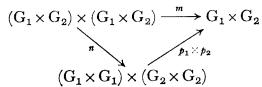
\includegraphics[keepaspectratio]{images/part002_baaabc67.jpg}}

where \(s(g, g') = (g', g)\) , \(m(g, g') = gg'\) , \(n(g, g') = g'g\) for all \(g\) , \(g'\) in \(G\) . This diagram is commutative. Hence \(n_*(t \otimes t') = m_*(s_*(t \otimes t')) = m_*(t' \otimes t)\) . This equality is precisely (i). Assertion (ii) follows from (i) and Proposition 6.

PROPOSITION 8. Let G, H be Lie groups and \(\phi\) a morphism of G into H. If \(t \in \mathcal{T}^{(\infty)}(G)\) , then \(\phi_{*}(t^{\vee}) = (\phi_{*}(t))^{\vee}\) .

Let \(\theta\) (resp. \(\theta'\) ) be the mapping \(g \mapsto g^{-1}\) of G into G (resp. of H into H). Then \(\phi \circ \theta = \theta' \circ \phi\) , whence \(\phi_*(\theta_*(t)) = \theta'_*(\phi_*(t))\) .

PROPOSITION 9. Let \(\mathrm{G}_1, \cdots, \mathrm{G}_n\) be Lie groups and \(\mathrm{G} = \mathrm{G}_1 \times \cdots \times \mathrm{G}_n\) . If the vector spaces \(\mathcal{T}^{(\infty)}(\mathrm{G})\) and \(\mathcal{T}^{(\infty)}(\mathrm{G}_1) \otimes \cdots \otimes \mathcal{T}^{(\infty)}(\mathrm{G}_n)\) are canonically identified, the algebra \(\mathcal{T}^{(\infty)}(\mathrm{G})\) is the tensor product of the algebras \(\mathcal{T}^{(\infty)}(\mathrm{G}_1), \ldots, \mathcal{T}^{(\infty)}(\mathrm{G}_n)\) . If \(t_i \in \mathcal{T}^{(\infty)}(\mathrm{G}_i)\) for \(i = 1, \ldots, n\) , then

\[
\left(t _ {1} \otimes \dots \otimes t _ {n}\right) ^ {\vee} = t _ {1} ^ {\vee} \otimes \dots \otimes t _ {n} ^ {\vee}.
\]

It suffices to consider the case \(n = 2\) . Let \(t_1, t_1'\) be in \(\mathcal{T}^{(\infty)}(\mathrm{G}_1)\) , \(t_2, t_2'\) in \(\mathcal{T}^{(\infty)}(\mathrm{G}_2)\) . We need to show that \((t_1 \otimes t_2) * (t_1' \otimes t_2') = (t_1 * t_1') \otimes (t_2 * t_2')\) and that \((t_1 \otimes t_2)^{\vee} = t_1^{\vee} \otimes t_2^{\vee}\) . Consider the diagram

\pandocbounded{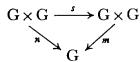
\includegraphics[keepaspectratio]{images/part002_69e6a490.jpg}}

where \(m((x_1, x_2), (x_1', x_2')) = (x_1x_1', x_2x_2')\) ,

\[
n ((x _ {1}, x _ {2}), (x _ {1} ^ {\prime}, x _ {2} ^ {\prime})) = ((x _ {1}, x _ {1} ^ {\prime}), (x _ {2}, x _ {2} ^ {\prime})),
\]

\(p_1(x_1, x_1') = x_1x_1', p_2(x_2, x_2') = x_2x_2'\) . This diagram is commutative. Hence

\[
m _ {*} \left(\left(t _ {1} \otimes t _ {2}\right) \otimes \left(t _ {1} ^ {\prime} \otimes t _ {2} ^ {\prime}\right)\right) = \left(p _ {1} \otimes p _ {2}\right) _ {*} \left(n _ {*} \left(\left(t _ {1} \otimes t _ {2}\right) \otimes \left(t _ {1} ^ {\prime} \otimes t _ {2} ^ {\prime}\right)\right)\right),
\]

that is

\[
\begin{array}{r l} (t _ {1} \otimes t _ {2}) * (t _ {1} ^ {\prime} \otimes t _ {2} ^ {\prime}) & = (p _ {1} \otimes p _ {2}) _ {*} ((t _ {1} \otimes t _ {1} ^ {\prime}) \otimes (t _ {2} \otimes t _ {2} ^ {\prime})) \\ & = p _ {1 *} (t _ {1} \otimes t _ {1} ^ {\prime}) \otimes p _ {2 *} (t _ {2} \otimes t _ {2} ^ {\prime}) \\ & = (t _ {1} * t _ {1} ^ {\prime}) \otimes (t _ {2} * t _ {2} ^ {\prime}). \end{array}
\]

It is seen analogously that \((t_1\otimes t_2)^\vee = t_1^\vee \otimes t_2^\vee\)

PROPOSITION 10. Let H be a Lie subgroup of G and \(i: \mathrm{H} \to \mathrm{G}\) the canonical injection. Then \(i_*\) is an injective homomorphism of the algebra \(\mathcal{T}^{(\infty)}(\mathrm{H})\) into the algebra \(\mathcal{T}^{(\infty)}(\mathrm{G})\) and \(i_*(t^\vee) = (i_*(t))^{\vee}\) for all \(t \in \mathcal{T}^{(\infty)}(\mathrm{H})\) .

This follows from Propositions 6 and 8 and Differentiable and Analytic Manifolds, R, 13.2.3.

\(\mathcal{T}^{(\infty)}(H)\) is identified with a subalgebra of \(\mathcal{T}^{(\infty)}(G)\) by means of the isomorphism of Proposition 10.

Remark. Proposition 10 remains valid if H is a Lie quasi-subgroup.

We recall (Differentiable and Analytic Manifolds, R, 13.5.1) that, if V is an analytic manifold over K, \(\mathcal{T}^{(\infty)}(\mathrm{V})\) has canonically a cogebra structure over K with a counit; the counit is the linear mapping of \(\mathcal{T}^{(\infty)}(\mathrm{G})\) into K which associates with each element of \(\mathrm{T}_x^{(\infty)}(\mathrm{V})\) its constant term.

PROPOSITION 11. Let G be a Lie group.

\begin{enumerate}
\def\labelenumi{(\roman{enumi})}
\item
  The cogebra \(\mathcal{T}^{(\infty)}(\mathbf{G})\) , with convolution, is a bigebra (Algebra, Chapter III, § 11, no. 4).
\item
  Let \(c\) be the coproduct on \(\mathcal{T}^{(\infty)}(\mathbf{G})\) . Let \(t \in \mathcal{T}^{(\infty)}(\mathbf{G})\) and write
\end{enumerate}

\[
c (t) = \sum_ {i = 1} ^ {n} t _ {i} \otimes t _ {i} ^ {\prime}.
\]

Then \(c(t^{\vee}) = \sum_{i=1}^{n} t_{i}^{\vee} \otimes t_{i}^{\prime\vee}\) .

We prove (i). In the definition of bigebras referred to, condition (1) follows from Propositions 2 and 3 and condition (2) follows from Differentiable and Analytic Manifolds, R, 13.5.1. Let \(d\) be the mapping \(g \mapsto (g, g)\) of G into \(\mathrm{G} \times \mathrm{G}\) . Then \(c = d_{*}\) and hence \(c\) is an algebra morphism (Propositions 6 and 9), which is condition (3). Let \(t \in \mathrm{T}_{g}^{\infty}(\mathrm{G})\) , \(t' \in \mathrm{T}_{g'}^{\infty}(\mathrm{G})\) have no constant term and \(\lambda\) , \(\lambda'\) be elements of K; then \(\varepsilon_{g} \otimes t'\) , \(t \otimes \varepsilon_{g'}\) , \(t \otimes t'\) are without constant term (Differentiable and Analytic Manifolds, R, 13.4.1) and hence the constant term of \((\lambda\varepsilon_{g} + t) * (\lambda' \varepsilon_{g'} + t')\) is \(\lambda\lambda'\) ; hence condition (4) holds.

We prove (ii). By Propositions 8 and 9,

\[
c (t ^ {\vee}) = d _ {*} (t ^ {\vee}) = (d _ {*} (t)) ^ {\vee} = \left(\sum_ {i = 1} ^ {n} t _ {i} \otimes t _ {i} ^ {\prime}\right) ^ {\vee} = \sum_ {i = 1} ^ {n} t _ {i} ^ {\prime \vee} \otimes t _ {i} ^ {\vee}.
\]

PROPOSITION 12. Let G, H be two Lie groups and \(\phi\) a morphism of G into H. Then \(\phi_{*}\) is a bigebra morphism of \(\mathcal{T}^{(\infty)}(G)\) into \(\mathcal{T}^{(\infty)}(H)\) .

This follows from Proposition 6 and Differentiable and Analytic Manifolds, R, 13.5.1.

Let \(G\) be a Lie group. The restrictions of the convolution and the coproduct to \(U(G)\) define a bigebra structure on \(U(G)\) . We have \(U(G)^{\vee} = U(G)\) . If \(\phi: G \to H\) is a Lie group morphism, we denote by \(U(\phi)\) the mapping \(t \mapsto \phi_{*}(t)\) of \(U(G)\) into \(U(H)\) ; this is a bigebra morphism. If \(\psi: H \to L\) is another Lie group morphism, then \(U(\psi \circ \phi) = U(\psi) \circ U(\phi)\) . If \(\phi\) is an immersion (resp. a submersion), \(U(\phi)\) is injective (resp. surjective) by Differentiable and Analytic Manifolds, R, 13.2.3. In particular, if \(H\) is a Lie subgroup of \(G\) , \(U(H)\) is identified with a subalgebra of \(U(G)\) , the coproduct on \(U(H)\) being the restriction of the coproduct on \(U(G)\) . If \(H\) is open in \(G\) , then \(U(H) = U(G)\) . If \(G_1, G_2\) are Lie groups, \(U(G_1 \times G_2)\) is identified with \(U(G_1) \times U(G_2)\) . The primitive elements of \(U(G)\) are those of \(T_e(G)\) (Differentiable and Analytic Manifolds, R, 13.5.3).

Again let \(\phi: \mathrm{G} \to \mathrm{H}\) be a Lie group morphism. If \(\operatorname{gr} \mathrm{U}(\mathrm{G})\) is identified \(\mathrm{TS}(\mathrm{T}_e(\mathrm{G}))\) and \(\operatorname{gr} \mathrm{U}(\mathrm{H})\) with \(\mathrm{TS}(\mathrm{T}_e(\mathrm{H}))\) , then \(\operatorname{gr} \mathrm{U}(\phi)\) is identified with \(\mathrm{TS}(\mathrm{T}_e(\phi))\) (Differentiable and Analytic Manifolds, R, 13.3.5). We apply this to the isomorphism \(g \mapsto g^{-1}\) of \(\mathrm{G}\) onto \(\mathrm{G}^{\vee}\) ; then \(\mathrm{T}_e(\phi) = -1\) and hence

\[
t \in \mathrm{U} _ {s} (\mathrm{G}) \Rightarrow t ^ {\vee} \equiv (- 1) ^ {s} t \bmod \mathrm{U} _ {s - 1} (\mathrm{G}).\tag{3}
\]

\subsection{CASE OF A GROUP OPERATING ON A MANIFOLD}

Let \(G\) be a Lie group, \(X\) a manifold of class \(C^r\) and \(f\) a law of left operation of class \(C^r\) of \(G\) on \(X\) . If \(t \in T_g^{(s)}(G)\) and \(u \in T_x^{(s')}(\mathbf{X})\) and \(s + s' \leqslant r\) , we denote by \(t * u\) the image of \(t \otimes u\) under \(f_*\) . We extend the product \(*\) to a bilinear mapping also denoted by *, of \(\mathcal{T}^{(s)}(G) \times \mathcal{T}^{(s')}(\mathbf{X})\) into \(\mathcal{T}^{(s+s')}(\mathbf{X})\) . Proposition 1 of no. 1 can be extended with obvious modifications to the present situation.

When G operates on itself by left translation, we recover Definition 1 of no. 1.

PROPOSITION 13. Let \(t \in \mathcal{T}^{(s)}(\mathbf{G})\) , \(t' \in \mathcal{T}^{(s')}(\mathbf{G})\) , \(u \in \mathcal{T}^{(s'')}(\mathbf{X})\) , such that

\[
s + s ^ {\prime} + s ^ {\prime \prime} \leqslant r.
\]

Then \((t*t')*u=t*(t'*u)\) .

This can be proved as is Proposition 2 of no. 1.

In particular, if \(r \leqslant \infty\) , the vector space \(\mathcal{T}^{(\infty)}(\mathbf{X})\) is a left module over the algebra \(\mathcal{T}^{(\infty)}(\mathbf{G})\) with the product \(*\) .

PROPOSITION 14. (i) Let \(g_0 \in G\) and \(\tau(g_0)\) be the mapping \(x \mapsto f(g_0, x)\) of \(X\) into \(X\) . If \(u \in \mathcal{T}^{(r)}(X)\) , then \(\tau(g_0)_*u = \varepsilon_{g_0} * u\) .

\begin{enumerate}
\def\labelenumi{(\roman{enumi})}
\setcounter{enumi}{1}
\tightlist
\item
  Let \(x_0 \in \mathbf{X}\) and \(\rho(x_0)\) be the mapping \(g \mapsto f(g, x_0)\) of \(G\) into \(X\) . If \(t \in T^{(r)}(G)\) , then \(\rho(x_0)_*t = t * \varepsilon_{x_0}\) .
\end{enumerate}

This can be proved as is Proposition 3 of no. 1.

In particular, if \(u \in \mathrm{T}(\mathrm{X})\) and \(t \in \mathrm{T}(\mathrm{G})\) , \(\varepsilon_{g_0} * u\) and \(t * \varepsilon_{x_0}\) are equal to the products \(g_0u\) and \(tx_0\) defined in § 2, no. 2.

PROPOSITION 15. Let G (resp. G') be a Lie group and X (resp. X') a manifold of class \(C^{r}\). Suppose that a law of left operation of class \(C^{r}\) of G (resp. G') on X (resp. X') is given. Let \(\phi\) be a morphism of G into G' and \(\psi\) a \(\phi\) -morphism of X into X'. Let \(t \in \mathcal{T}^{(s)}(G)\) , \(u \in \mathrm{T}^{(s')}(\mathrm{X})\) be such that \(s + s' \leqslant r\) . Then

\[
\psi_ {*} (t * u) = \phi_ {*} (t) * \psi_ {*} (u).
\]

This can be proved as is Proposition 6 of no. 2.

Remark. Let \(f\) be a law of right operation of class \(\mathbf{C}^r\) of \(\mathbf{G}\) on \(\mathbf{X}\) . If \(t \in \mathcal{T}^{(s)}(\mathbf{G})\) and \(u \in \mathcal{T}^{(s')}(\mathbf{X})\) , with \(s + s' \leqslant r\) , we denote by \(u * t\) the image of \(u \otimes t\) under \(f_*\) . Propositions 13, 14, 15 go over to this situation in an obvious way.

PROPOSITION 16. Let G, G' be Lie groups, X a manifold of class \(C^{r}\) and suppose that G (resp. G') operates on X on the left (resp. right), with \((gx)g' = g(xg')\) for all \(x \in X\) , \(g \in G\) , \(g' \in G'\) . Let \(t \in \mathcal{T}^{(s)}(G)\) , \(t' \in \mathcal{T}^{(s')}(\mathrm{G}')\) , \(t'' \in \mathrm{T}^{(s'')}(\mathrm{X})\) , with \(s + s' + s'' \leqslant r\) . Then

\[
(t * t ^ {\prime \prime}) * t ^ {\prime} = t * (t ^ {\prime \prime} * t ^ {\prime}).
\]

\((t*t'')*t'\) (resp. \(t*(t''*t')\) ) is the image of \(t\otimes t''\otimes t'\) under the mapping \((g,x,g')\mapsto(gx)g'\) (resp. \(g(xg')\) ) of G × X × G' into X.

\subsection{CONVOLUTION OF POINT DISTRIBUTIONS AND FUNCTIONS}

Let G be a Lie group, X a manifold of class \(C^{r}\) and \((g, x) \mapsto gx\) a law of left operation of class \(C^{r}\) of G on X. For all \(x \in X\) , let \(\rho(x)\) denote the orbital mapping of x.

DEFINITION 3. Let \(t \in \mathcal{T}^{(s)}(\mathrm{G})\) with \(s \leqslant r\) . Let \(f: \mathrm{X} \to \mathrm{F}\) be a function of class \(\mathbf{C}^r\) with values in a Hausdorff polynormed space (for example \(\mathrm{F} = \mathrm{K}\) ). The convolution of \(t\) and \(f\) , denoted by \(t * f\) , is the function on \(\mathbf{X}\) with values in \(\mathrm{F}\) defined by

\[
(t * f) (x) = \langle t ^ {\vee} * \varepsilon_ {x}, f \rangle .
\]

Then

\[
\begin{array}{l l} (t * f) (x) = \langle \rho (x) _ {*} (t ^ {\vee}), f \rangle & (\text {no. 3, Proposition 14 (ii)}) \\ = \langle t ^ {\vee}, f \circ \rho (x) \rangle & (Diff. \& Anal. Man., R, 13.2.3) \\ = \langle t, (f \circ \rho (x)) ^ {\vee} \rangle & (Diff. \& Anal. Man., R, 13.2.3). \end{array}\tag{4}
\]

Note that Definition 3 can also be written in the more symmetric form

\[
\langle \varepsilon_ {x}, t * f \rangle = \langle t ^ {\vee} * \varepsilon_ {x}, f \rangle .\tag{5}
\]

The function \((g,x)\mapsto f(gx) = (f\circ \rho (x))(g)\) on \(\mathbf{G}\times \mathbf{X}\) is of class \(\mathbf{C}^r\) . By Differentiable and Analytic Manifolds, R, 13.4.4, the function \(x\mapsto \langle t^\vee,f\circ \rho (x)\rangle\) is therefore of class \(\mathbf{C}^{r - s}\) if \(s < \infty\) . In other words, if \(s < \infty\) , \(t*f\) is of class \(\mathbf{C}^{r - s}\) .

Clearly \(t * f\) depends linearly on \(t\) and \(f\) .

Formula (4) implies in particular, for \(g \in G\) ,

\[
\left(\varepsilon_ {g} * f\right) (x) = f \left(g ^ {- 1} x\right)\tag{6}
\]

that is

\begin{enumerate}
\def\labelenumi{(\arabic{enumi})}
\setcounter{enumi}{6}
\tightlist
\item
\end{enumerate}

\[
\varepsilon_ {g} * f = \gamma (g) f.
\]

Suppose that \(\mathbf{K} = \mathbf{R}\) or \(\mathbf{C}\) , that \(\mathbf{G}\) and \(\mathbf{X}\) are finite-dimensional and that \(\mathbf{X}\) has a positive measure invariant under \(\mathbf{G}\) . The definition of \(\varepsilon_g * f\) agrees with that of Integration, Chapter VIII, § 4, no. 1 (cf.~formula (2), loc. cit.).

PROPOSITION 17. Let \(t \in \mathcal{T}^{(s)}(\mathrm{G})\) , \(t' \in \mathcal{T}^{(s')}(\mathrm{X})\) and \(f: X \to \mathrm{F}\) a function of class \(\mathbf{C}^{r}\) with \(s + s' \leqslant r\) . Then

\[
\langle t ^ {\prime}, t * f \rangle = \langle t ^ {\vee} * t ^ {\prime}, f \rangle .
\]

\[
\begin{array}{l l} \langle t ^ {\prime}, t * f \rangle = \langle t ^ {\prime}, x \mapsto \langle t, g \mapsto f (g ^ {- 1} x) \rangle \rangle & \text { by   (4) } \\ = \langle t \otimes t ^ {\prime}, (g, x) \mapsto f (g ^ {- 1} x) \rangle & \text {(Diff. \& Anal. Man., R, 13.4.4)} \\ = \langle t ^ {\vee} \otimes t ^ {\prime}, (g, x) \mapsto f (g x) \rangle & \text {(Diff. \& Anal. Man., R, 13.2.3)} \\ = \langle t ^ {\vee} * t ^ {\prime}, f \rangle . \end{array}
\]

PROPOSITION 18. Let \(t \in \mathcal{T}^{(s)}(\mathrm{G})\) , \(t' \in \mathcal{T}^{(s')}(\mathrm{G})\) and \(f: \mathrm{X} \to \mathrm{F}\) a function of class \(\mathbf{C}^r\) , with \(s + s' \leqslant r\) . Then

\[
(t * t ^ {\prime}) * f = t * (t ^ {\prime} * f).
\]

For all \(x \in X\) ,

\[
\begin{array}{l l} \langle \varepsilon_ {x}, (t * t ^ {\prime}) * f \rangle = \langle (t * t ^ {\prime}) ^ {\vee} * \varepsilon_ {x}, f \rangle & \text {by (5)} \\ = \langle t ^ {\prime \vee} * (t ^ {\vee} * \varepsilon_ {x}), f \rangle & \text {(Propositions 2 and 7)} \\ = \langle t ^ {\vee} * \varepsilon_ {x}, t ^ {\prime} * f \rangle & \text {(Proposition 17)} \\ = \langle \varepsilon_ {x}, t * (t ^ {\prime} * f) \rangle & \text {(Proposition 17).} \end{array}
\]

If \(r \geqslant \infty\) , we see that the set of functions of class \(C^\infty\) on \(X\) with values in \(F\) is a left module over the algebra \(\mathcal{T}^{(\infty)}(G)\) .

PROPOSITION 19. Let \(t \in \mathcal{T}^{(s)}(\mathrm{G})\) , with \(s \leqslant r\) . Let \(f\) (resp. \(f'\) ) be a function of class \(\mathrm{C}^r\) on \(\mathbf{X}\) with values in a Hausdorff polynormed space \(\mathrm{F}\) (resp. \(\mathrm{F}'\) ). Let \((u, u') \mapsto uu'\) be a continuous bilinear mapping of \(\mathrm{F} \times \mathrm{F}'\) into a Hausdorff polynormed space \(\mathrm{F}''\) , so that \(ff'\) is a function of class \(\mathrm{C}^r\) on \(\mathbf{X}\) with values in \(\mathrm{F}''\) . Let \(\sum_{i=1}^{n} t_i \otimes t_i'\) be the image of \(t\) in \(\mathcal{T}^{(s)}(\mathrm{G}) \otimes \mathcal{T}^{(s)}(\mathrm{G})\) under the coproduct. Then

\[
t * (f f ^ {\prime}) = \sum_ {i = 1} ^ {n} (t _ {i} * f) (t _ {i} ^ {\prime} * f ^ {\prime}).
\]

Let \(x \in X\) and let \(\rho(x)\) denote the orbital mapping of x. Then

\[
\begin{array}{l l} \langle \varepsilon_ {x}, t * (f f ^ {\prime}) \rangle = \langle t ^ {\vee}, (f f ^ {\prime}) \circ \rho (x) \rangle & \text {by (4)} \\ = \langle t ^ {\vee}, (f \circ \rho (x)) (f ^ {\prime} \circ \rho (x)) \rangle \\ = \sum_ {i = 1} ^ {n} \langle t _ {i} ^ {\vee}, f \circ \rho (x) \rangle \langle t _ {i} ^ {\prime \vee}, f ^ {\prime} \circ \rho (x) \rangle \\ & (\text {Diff. \& Man. Anal., R, 13.5.2}) \\ = \sum_ {i = 1} ^ {n} \langle \varepsilon_ {x}, t _ {i} * f \rangle \langle \varepsilon_ {x}, t _ {i} ^ {\prime} * f ^ {\prime} \rangle & \text {by (4).} \end{array}
\]

Remark 1. Let G be a Lie group, X a manifold of class \(\mathbf{C}^r\) and \((x,g)\mapsto xg\) a law of right operation of class \(\mathbf{C}^r\) of G on X. If \(t\in \mathcal{T}^{(s)}(\mathrm{G})\) with \(s\leqslant r\) and \(f\colon \mathrm{X}\to \mathrm{F}\) is a function of class \(\mathbf{C}^r\) on X, we denote by \(f*t\) the function on X defined by

\[
\begin{array}{r l} \langle \varepsilon_ {x}, f * t \rangle & = \langle \varepsilon_ {x} * t ^ {\vee}, f \rangle \\ & = \langle \rho (x) _ {*} (t ^ {\vee}), f \rangle \\ & = \langle t ^ {\vee}, f \circ \rho (x) \rangle \\ & = \langle t, (f \circ \rho (x)) ^ {\vee} \rangle . \end{array}\tag{8}
\]

In particular

\[
(f * \varepsilon_ {g}) (x) = f (x g ^ {- 1})\tag{9}
\]

that is

\[
f * \varepsilon_ {g} = \delta (g) ^ {- 1} f.\tag{10}
\]

Propositions 17, 18, 19 become, in the obvious notation,

\begin{enumerate}
\def\labelenumi{(\arabic{enumi})}
\setcounter{enumi}{10}
\tightlist
\item
\end{enumerate}

\[
\langle t ^ {\prime}, f * t \rangle = \langle t ^ {\prime} * t ^ {\vee}, f \rangle\tag{11}
\]

\[
f * (t * t ^ {\prime}) = (f * t) * t ^ {\prime}\tag{12}
\]

\[
(f f ^ {\prime}) * t = \sum_ {i = 1} ^ {n} (f * t _ {i}) (f ^ {\prime} * t _ {i} ^ {\prime}).\tag{13}
\]

PROPOSITION 20. Let \(G\) , \(G'\) be Lie groups, \(X\) a manifold of class \(C^r\) and \((g, x) \mapsto gx\) (resp. \((x, g') \mapsto xg'\) ) a law of left (resp. right) operation of class \(C^r\) of \(G\) (resp. \(G'\) ) on \(X\) . Suppose that \((gx)g' = g(xg')\) for all \(x \in X\) , \(g \in G\) , \(g' \in G'\) . Let \(t \in \mathcal{T}^{(s)}(G)\) , \(t' \in \mathcal{T}^{(s')}(\mathrm{G}')\) and \(f: X \to F\) be a function of class \(C^r\) such that \(s + s' \leqslant r\) . Then

\[
(t * f) * t ^ {\prime} = t * (f * t ^ {\prime}).
\]

For all \(x \in X\) ,

\[
\begin{array}{l l} \langle \varepsilon_ {x}, (t * f) * t ^ {\prime} \rangle = \langle \varepsilon_ {x} * t ^ {\prime \vee}, t * f \rangle & \text { by   (8) } \\ = \langle t ^ {\vee} * (\varepsilon_ {x} * t ^ {\prime \vee}), f \rangle & \text {(Proposition 17)} \\ = \langle t ^ {\vee} * \varepsilon_ {x}, f * t ^ {\prime} \rangle & \text {(Proposition 2 and (11))} \\ = \langle \varepsilon_ {x}, t * (f * t ^ {\prime}) \rangle & \text { by   (5). } \end{array}
\]

In particular, consider G as operating on itself by left and right translations. If \(f \colon \mathbf{G} \to \mathbf{F}\) is a function of class \(\mathbf{C}^r\) on G and \(t \in \mathcal{T}^{(s)}(\mathbf{G})\) (with \(s \leqslant r\) ), \(t * f\) and \(f * t\) are, if \(s < \infty\) , functions of class \(\mathbf{C}^{r - s}\) on G. Further, let \(t' \in \mathcal{T}^{(s')}(\mathbf{G})\) , with \(s + s' \leqslant r\) . Then

\[
(t * f) * t ^ {\prime} = t * (f * t ^ {\prime}).\tag{14}
\]

In particular, \(\mathcal{C}^{\infty}(\mathrm{G})\) is a \((\mathcal{T}^{(\infty)}(\mathrm{G}),\mathcal{T}^{(\infty)}(\mathrm{G}))\) -bimodule. Formulae (5) and (8) admit as special cases

\[
\langle t, f \rangle = \left\langle \varepsilon_ {e}, t ^ {\vee} * f \right\rangle = \left\langle \varepsilon_ {e}, f * t ^ {\vee} \right\rangle .\tag{15}
\]

Remark 2. Let \((g,x)\mapsto gx\) be a law of left operation of class \(\mathbf{C}^r\) of \(G\) on \(X\) . Let \(t\in \mathbf{U}_s(\mathbf{G})\) with \(s\leqslant r\) , \(\Omega\) be an open subset of \(X\) and \(f\colon \Omega \to F\) a function of class \(\mathbf{C}^r\) . \(t*f\) can also be defined by formula (4) or (5); it is a function defined on \(\Omega\) with values in \(F\) , of class \(\mathbf{C}^{r - s}\) if \(s < \infty\) . The results of this no. extend in an obvious way to this situation.

\subsection{FIELDS OF POINT DISTRIBUTIONS DEFINED BY THE ACTION OF A GROUP ON A MANIFOLD}

Let \((g,x)\mapsto\lambda(g,x)=gx\) be a law of left operation of class \(C^{r}\) of G on X. Let \(s\leqslant r\) and \(t\in U_{s}(G)\) . For all \(x\in X\) , \(t*\varepsilon_{x}\in T_{x}^{(s)}(X)\) . The mapping \(x\mapsto t*\varepsilon_{x}\) is called the field of point distributions defined by t and the action of G on X and denoted sometimes by \(D_{t}^{\lambda}\) or simply \(D_{t}\) . Let \(\Omega\) be an open subset of X and F a Hausdorff polynormed space. If \(f\colon\Omega\to F\) is of class \(C^{r}\) and \(s\leqslant r\) , the function \(t^{\vee}\ast f\) on \(\Omega\) is also denoted by \(D_{t}.f\) . Then

\[
(D _ {t} f) (x) = \langle t * \varepsilon_ {x}, f \rangle .\tag{16}
\]

If \(s < \infty\) , then \(D_t f \in \mathcal{C}^{r-s}(\Omega, F)\) by no. 4. Thus \(f \mapsto D_t f\) is a mapping of \(\mathcal{C}^r(\Omega, F)\) into \(\mathcal{C}^{r-s}(\Omega, F)\) (often denoted by \(D_t\) by an abuse of notation).

If \(t \in \mathrm{U}_s(\mathrm{G})\) , \(t' \in \mathrm{U}_{s'}(\mathrm{G})\) and \(s + s' \leqslant r\) , then, by Proposition 18 of no. 4,

\[
\mathrm{D} _ {t * t ^ {\prime}} f = \mathrm{D} _ {t ^ {\prime}} (\mathrm{D} _ {t} f)\tag{17}
\]

and hence, using the abuse of notation indicated above,

\[
\mathrm{D} _ {t * t ^ {\prime}} = \mathrm{D} _ {t ^ {\prime}} \circ \mathrm{D} _ {t}.\tag{18}
\]

Suppose that G and X are finite-dimensional. The mapping \((t, x) \mapsto t \otimes \varepsilon_{x}\) of \(\mathrm{T}^{(\mathrm{s})}(\mathrm{G}) \times \mathrm{X}\) into the vector bundle \(\mathrm{T}^{(\mathrm{s})}(\mathrm{G} \times \mathrm{X})\) (cf.~Differentiable and Analytic Manifolds, R, 13.2.5) is of class \(C^{r-s}\) . Hence (Differentiable and Analytic Manifolds, R, 13.2.5) the mapping \((t, x) \mapsto t * \varepsilon_{x}\) of \(\mathrm{T}^{(\mathrm{s})}(\mathrm{G}) \times \mathrm{X}\) into the vector bundle \(\mathrm{T}^{(\mathrm{s})}(\mathrm{X})\) is of class \(C^{r-s}\) . In particular, \(D_{t}\) is a differential operator of order \(\leqslant s\) and class \(C^{r-s}\) in the sense of Differentiable and Analytic Manifolds, R, 14.1.6. By formula (16), the function \(D_{t}f\) is then the image of f under this differential operator (Differentiable and Analytic Manifolds, R, 14.1.4).

We now no longer suppose that G and X are finite-dimensional. Let \(\psi\) be an automorphism of the manifold X and \(\Delta\) a field of point distributions on X. Conforming with the general definitions, the transform of \(\Delta\) under \(\psi\) is the field of point distributions on X whose value at \(\psi(x)\) is \(\psi_{*}(\Delta(x))\) ; we denote this mapping by \(\psi(\Delta)\) . If \(g \in G\) and \(\tau(g)\) denotes the automorphism \(x \mapsto gx\) of X, the transform of \(\Delta\) under \(\tau(g)\) is also called the transform of \(\Delta\) under g.

PROPOSITION 21. Let \(\psi\) be an automorphism of X commuting with the operations of G. Then \(D_{t}\) is invariant under \(\psi\) .

For all \(x \in X\) ,

\[
\begin{array}{r l} (\psi (\mathrm{D} _ {t})) (\psi (x)) & = \psi_ {*} (\mathrm{D} _ {t} (x)) = \psi_ {*} (t * \varepsilon_ {x}) \\ & = t * \psi_ {*} (\varepsilon_ {x}) \quad \text {(Proposition 15)} \\ & = t * \varepsilon_ {\psi (x)} = \mathrm{D} _ {t} (\psi (x)). \end{array}
\]

PROPOSITION 22. If \(g \in G\) , the transform of \(D_t\) under \(g\) is \(D_{\varepsilon_g * t * \varepsilon_{g^{-1}}}\) .

The value of this transform at gx is

\[
\begin{array}{r l r} \tau (g) _ {*} (\mathrm{D} _ {t} (x)) & = \tau (g) _ {*} (t * \varepsilon_ {x}) \\ & = \varepsilon_ {g} * (t * \varepsilon_ {x}) & \text {(Proposition 14 (i))} \\ & = (\varepsilon_ {g} * t * \varepsilon_ {g^{-1}}) * \varepsilon_ {g x} & \text {(Propositions 1 and 2)} \\ & = \mathrm{D} _ {\varepsilon_ {g} * t * \varepsilon_ {g^{-1}}} (g x). \end{array}
\]

Let \((x,g)\mapsto \mu (x,g) = xg\) be a law of right operation of class \(\mathbf{C}^r\) of G on X. Let \(s\leqslant r\) and \(t\in \mathrm{U}_{s}(\mathrm{G})\) . For all \(x\in \mathbf{X}\) , \(\varepsilon_{x}*t\in \mathrm{T}_{x}^{(s)}(\mathbf{X})\) . The mapping \(x\mapsto \varepsilon_x*t\) is called the field of distributions defined by \(t\) and the action of G on X and is sometimes denoted by \(\mathrm{D}_{t}^{\mu}\) or simply \(\mathrm{D}_t\) . Let \(\Omega\) be an open subset of X. If \(f:\Omega \to F\) is of class \(\mathbf{C}^r\) , the function \(f*t^{\vee}\) is denoted by \(\mathrm{D}_t f\) . Then

\[
\left(\mathrm{D} _ {t} f\right) (x) = \langle \varepsilon_ {x} * t, f \rangle\tag{19}
\]

and, in the obvious notation,

\begin{enumerate}
\def\labelenumi{(\arabic{enumi})}
\setcounter{enumi}{19}
\tightlist
\item
\end{enumerate}

\[
D _ {t * t ^ {\prime}} f = \mathrm{D} _ {t} (\mathrm{D} _ {t ^ {\prime}} f)\tag{20}
\]

\[
\mathrm{D} _ {t * t ^ {\prime}} = \mathrm{D} _ {t} \circ \mathrm{D} _ {t ^ {\prime}}\tag{21}.
\]

Proposition 21 remains valid. Let \(g \in G\) . The transform of \(D_t\) under \(g\) (that is under the automorphism \(x \mapsto xg\) of \(X\) ) is \(D_{\varepsilon_{g^{-1}} * t * \varepsilon_g}\) .

\subsection{INVARIANT FIELDS OF POINT DISTRIBUTIONS ON A LIE GROUP}

DEFINITION 4. Let G be a Lie group. A field of distributions on G is called left (resp. right) invariant if it is invariant under left (resp. right) translations of G.

In other words, a field of distributions \(g \mapsto \Delta_g\) on \(G\) is left invariant if

\[
\Delta_ {g g ^ {\prime}} = \gamma (g) _ {*} \Delta_ {g ^ {\prime}} \quad \text { for } g, g ^ {\prime} \text { in } G,
\]

or again if

\[
\Delta_ {g g ^ {\prime}} = \varepsilon_ {g} * \Delta_ {g ^ {\prime}} \quad \text { for   } g, g ^ {\prime} \text {   in   G. }
\]

It is right invariant if

\[
\Delta_ {g g ^ {\prime}} = \delta (g ^ {\prime - 1}) _ {*} \Delta_ {g} \quad \text { for   } g, g ^ {\prime} \text {   in   G },
\]

or again if.

\[
\Delta_ {g g ^ {\prime}} = \Delta_ {g} * \varepsilon_ {g ^ {\prime}}, \quad \text { for   } g, g ^ {\prime} \text {   in   G. }
\]

DEFINITION 5. Let G be a Lie group and \(t \in \mathrm{U}(\mathrm{G})\) . Let \(\mathbf{L}_t\) denote the field of distributions \(g \mapsto \varepsilon_g * t\) on G and \(\mathbb{R}_t\) the field of distributions \(g \mapsto t * \varepsilon_g\) on G.

In other words, \(L_{t}\) (resp. \(R_{t}\) ) is the field of distributions defined by t and G operating on G on the right (resp. left) by means of the mapping \((g, g') \mapsto gg'\) . Let \(\Omega\) be an open subset of G and F a Hausdorff polynormed space; if \(f \in \mathcal{C}^{\omega}(\Omega, \mathrm{F})\) , then \(\mathrm{L}_{t}f = f * t^{\vee} \in \mathcal{C}^{\omega}(\Omega, \mathrm{F})\) and

\[
\mathrm{R} _ {t} f = t ^ {\vee} * f \in \mathcal {C} ^ {\omega} (\Omega , \mathrm{F})
\]

(no. 5). If G is finite-dimensional, the differential operators \(L_{t}\) and \(R_{t}\) are of class \(C^{\omega}\) (no. 5).

PROPOSITION 23. (i) The mapping \(t \mapsto \mathbf{L}_t\) (resp. \(t \mapsto \mathbf{R}_t\) ) is an isomorphism of the vector space \(\mathbf{U}(\mathbf{G})\) onto the vector field of left (resp. right) invariant distributions on \(\mathbf{G}\) .

\begin{enumerate}
\def\labelenumi{(\roman{enumi})}
\setcounter{enumi}{1}
\item
  For \(t, t'\) in U(G), \(L_{t*t'} = L_t \circ L_{t'}\) , \(R_{t*t'} = R_{t'} \circ R_t\) , \(L_t \circ R_{t'} = R_{t'} \circ L_t\) (with the abuse of notation of no. 5).
\item
  If \(\theta\) is the mapping \(g \mapsto g^{-1}\) of \(\mathbf{G}\) onto \(\mathbf{G}\) , then \(\theta(\mathbf{L}_t) = \mathbf{R}_{t^{\vee}}\) .
\item
  If \(t \in \mathrm{U}(\mathrm{G})\) and \(g \in \mathrm{G}\) , then \((\mathrm{L}_t)_g = (\mathrm{R}_{\varepsilon_g * t * \varepsilon_{g^{-1}}})_g\) .
\end{enumerate}

In G every right translation commutes with every left translation. By Proposition 21 of no. 5, \(L_{t}\) is therefore left invariant. As \((\mathbf{L}_{t})_{e}=t\) , the mapping \(t\mapsto L_{t}\) is injective. Let \(\Delta\) be a field of left invariant distributions on G; let \(t=\Delta_{e}\) ; then \(\Delta\) and \(L_{t}\) have the same value at e and are left invariant and hence \(\Delta=L_{t}\) . This proves (i) for \(L_{t}\) and the argument is similar for \(R_{t}\) . The formulae \(L_{t*t^{\prime}}=L_{t}\circ L_{t^{\prime}}\) , \(R_{t*t^{\prime}}=R_{t^{\prime}}\circ R_{t}\) follow from (21) and (18). Let \(t\in\mathrm{U}_{s}(\mathrm{G})\) , \(t^{\prime}\in\mathrm{U}_{s^{\prime}}(\mathrm{G}), f\in\mathcal{C}^{r}(\Omega,\mathrm{F})\) , where \(\Omega\) is open in G and \(s+s^{\prime}\leqslant r\) ; then

\[
\begin{array}{r l} \mathrm{L} _ {t} \mathrm{R} _ {t ^ {\prime}} f & = \mathrm{L} _ {t} (t ^ {\prime^ {\vee}} * f) = (t ^ {\prime^ {\vee}} * f) * t \\ & = t ^ {\prime^ {\vee}} * (f * t ^ {\vee}) \quad \text {(Proposition 20)} \\ & = \mathrm{R} _ {t ^ {\prime}} \mathrm{L} _ {t} f \end{array}
\]

and hence \(\mathbf{L}_t\circ \mathbf{R}_{t'} = \mathbf{R}_{t'}\circ \mathbf{L}_t\) . As \(\theta\) is an isomorphism of \(\mathbf{G}\) onto \(\mathbf{G}^{\vee}\) , \(\theta (\mathrm{L}_t)\) is a field of right invariant distributions on \(\mathbf{G}\) ; its value at \(e\) is \(\theta^{*}(t) = t^{\vee}\) hence \(\theta (\mathrm{L}_t) = \mathrm{R}_{t^{\vee}}\) . Finally,

\[
\left(\mathrm{L} _ {t}\right) _ {g} = \varepsilon_ {g} * t = \left(\varepsilon_ {g} * t * \varepsilon_ {g^{-1}}\right) * \varepsilon_ {g} = \left(\mathrm{R} _ {\varepsilon_ {g} * t * \varepsilon_ {g^{-1}}}\right) _ {g}.
\]

Remark 1. It is the action of G on itself by right translation which defines the fields of left invariant distributions.

Remark 2. Suppose that G is finite-dimensional. The mapping

\[
(t, g) \mapsto (\mathbf {R} _ {t}) _ {g} = t * \varepsilon_ {g}
\]

of \(\mathrm{U}_{s}(\mathrm{G})\times\mathrm{G}\) into \(\mathrm{T}^{(s)}(\mathrm{G})\) is an isomorphism of analytic vector bundles; for this mapping is bijective, linear on each fibre and analytic (no. 5); on the other hand, let \(\phi:\mathrm{T}^{(s)}(\mathrm{G})\to\mathrm{U}_{s}(\mathrm{G})\times\mathrm{G}\) be the inverse bijection; if \(t\in\mathrm{T}_{g}^{(s)}(\mathrm{G})\) , then \(\phi(t)=(t*\varepsilon_{g^{-1}},g)\) and hence \(\phi\) is analytic. The isomorphism \(\phi\) is called the right trivialization of \(\mathrm{T}^{(s)}(\mathrm{G})\) . Similarly, consider the mapping \((t,g)\mapsto(\mathrm{L}_{\mathrm{t}})_{g}=\varepsilon_{g}*t\) of \(\mathrm{U}_{s}(\mathrm{G})\times\mathrm{G}\) into \(\mathrm{T}^{(s)}(\mathrm{G})\) ; the inverse isomorphism is called the left trivialization of \(\mathrm{T}^{(s)}(\mathrm{G})\) . By restriction we recover the right and left trivializations of \(\mathrm{T}(\mathrm{G})\) (§2, no. 2).

\subsection{LIE ALGEBRA OF A LIE GROUP}

Let \(\mathbf{G}\) be a Lie group. In \(\mathrm{U}(\mathbf{G})\) , as in any associative algebra, we write \([t, t'] = t * t' - t' * t\) . As \(\mathrm{T}_{e}(\mathbf{G})\) is the set of primitive elements of \(\mathrm{U}(\mathbf{G})\) , \([\mathrm{T}_{e}(\mathbf{G}), \mathrm{T}_{e}(\mathbf{G})] \subset \mathrm{T}_{e}(\mathbf{G})\) (Chapter II, § 1, no. 2, Proposition 4). The restriction of the bracket to \(\mathrm{T}_{e}(\mathbf{G})\) therefore defines on \(\mathrm{T}_{e}(\mathbf{G})\) a Lie algebra structure.

Lemma 1. Let \(\mathbf{X}\) and \(\mathbf{X}'\) be complete normable spaces, \(\mathbf{X}_0\) an open neighbourhood of 0 in \(\mathbf{X}\) and \(f\) an analytic mapping of \(\mathbf{X}_0\) into \(\mathbf{X}'\) such that \(f(0) = 0\) . Let \(f = f_1 + f_2 + f_3 + \dots\) be the expansion of \(f\) as an integral series about 0, where \(f_i\) is a homogeneous continuous-polynomial of degree \(i\) on \(\mathbf{X}\) with values in \(\mathbf{X}'\) . Let \(t\) be an element of \(\mathrm{TS}^2 (\mathbf{X})\) , considered as a point distribution on \(\mathbf{X}\) with support contained in \(\{0\}\) . Let \(t' = f_{\star}(t) \in \mathrm{TS}(\mathbf{X}')\) . The homogeneous component of \(t'\) of degree 1 is \(\langle f_2, t \rangle\) .

Let \(t_{1}^{\prime}\) be this component. Then, for every continuous linear mapping u of \(X^{\prime}\) into a polynormed space,

\[
\begin{array}{l l} u (t _ {1} ^ {\prime}) = \langle t ^ {\prime}, u \rangle & \text { because   } u \text {   is   continuous   and   linear } \\ = \langle t, u \circ f \rangle & (\text { Diff.   \&   Anal.   Man.,   R,   13.2.3 }) \\ = \langle t, u \circ f _ {2} \rangle & \text { because   } t \in \mathsf {T S} ^ {2} (\mathbf {X}) \\ = u (\langle t, f _ {2} \rangle) & (\text { Diff.   \&   Anal.   Man.,   R,   13.2.2 }), \end{array}
\]

whence the lemma.

PROPOSITION 24. Let G be a Lie group and (U, \(\phi\) , E) a chart on G such that \(\phi(e) = 0\) . Let V be an open neighbourhood of \(e\) such that \(\mathrm{V}^2 \subset \mathrm{U}\) . Let \(m\) be the analytic mapping \((a, b) \mapsto \phi(\phi^{-1}(a)\phi^{-1}(b))\) of \(\phi(V) \times \phi(V)\) into E. Let

\[
m = \sum_ {i, j \geqslant 0} m _ {i, j}
\]

be the expansion of \(m\) as an integral series about \((0,0)\) , where \(m_{i,j}\) is a bihomogeneous continuous-polynomial of bidegree \((i,j)\) on \(\mathbf{E} \times \mathbf{E}\) with values in \(\mathbf{E}\) .

\begin{enumerate}
\def\labelenumi{(\roman{enumi})}
\item
  \(m_{i,0} = m_{0,j} = 0\) for all \(i \neq 1\) and \(j \neq 1\) .
\item
  \(m_{1,0}(a,b)=a\) and \(m_{0,1}(a,b)=b\) for all \(a\in E\) , \(b\in E\) .
\item
  Let \(\psi: \mathrm{T}_e(\mathrm{G}) \to \mathrm{E}\) be the differential of \(\phi\) at \(e\) . For all \(u, v\) in \(\mathrm{T}_e(\mathrm{G})\) ,
\end{enumerate}

\[
\psi ([ u, v ]) = m _ {1, 1} (\psi (u), \psi (v)) - m _ {1, 1} (\psi (v), \psi (u)).
\]

\(m(a,0) = a\) , \(m(0,b) = b\) for all \(a\) , \(b\) in \(\phi (\mathrm{V})\) , which proves (i) and (ii). Let \(u, v\) be in \(\mathrm{T_e(G)}\) . Let \(\mathrm{T_0(E)}\) be identified with E and hence \(\psi\) with \(\mathrm{T_e}(\phi)\) . The images of \(u\) and \(v\) under \(\mathrm{T_e}(\phi)\) are \(\psi (u)\) and \(\psi (v)\) . The tensor product point distribution of these images is the symmetric product of \((\psi(u),0)\) and \((0,\psi (v))\) in \(\mathsf{TS(E\times E)} = \mathsf{TS(E)}\times \mathsf{TS(E)}\) , that is

\[
(\psi (u), 0) \otimes (0, \psi (v)) + (0, \psi (v)) \otimes (\psi (u), 0).
\]

Hence \(\phi_{*} (u * v)\) is the image of the above element under the mapping \(m\) of \(\phi(V) \times \phi(V)\) into \(E\) . Its component of degree 1 in TS(E) is, by Lemma 1,

\[
x = \langle m _ {1, 1}, (\psi (u), 0) \otimes (0, \psi (v)) + (0, \psi (v)) \otimes (\psi (u), 0) \rangle .
\]

We define a bilinear mapping \(n\colon (\mathbf{E}\times \mathbf{E})^2\to \mathbf{E}\) by

\[
n ((a, b), (a ^ {\prime}, b ^ {\prime})) = m _ {1, 1} (a, b ^ {\prime}).
\]

Then \(n((a, b), (a, b)) = m_{1,1}(a, b)\) and hence

\[
\begin{array}{l} x = \langle n, (\psi (u), 0) \otimes (0, \psi (v)) + (0, \psi (v)) \otimes (\psi (u), 0) \rangle \\ \quad = m _ {1, 1} (\psi (u), \psi (v)) + m _ {1, 1} (0, 0) = m _ {1, 1} (\psi (u), \psi (v)). \end{array}
\]

Similarly, \(\phi_{*} (v * u)\) admits \(m_{1,1}(\phi(v), \phi(u))\) as component of degree 1 in TS(E). As \(\phi([u, v])\) is of degree 1, this proves (iii).

COROLLARY. The normable space \(\mathrm{T}_e(\mathrm{G})\) together with the bracket, is a normable Lie algebra.

DEFINITION 6. The normable space \(\mathrm{T_e(G)}\) , together with the bracket, is called the normable Lie algebra of \(\mathbf{G}\) , or simply the Lie algebra of \(\mathbf{G}\) , and is denoted by \(\mathbf{L(G)}\) .

PROPOSITION 25. Let \(\mathbf{G}\) be a Lie group and \(\operatorname{E}(\mathbf{G})\) the enveloping algebra of \(\mathbf{L}(\mathbf{G})\) . The canonical injection of \(\mathbf{L}(\mathbf{G})\) into \(\operatorname{E}(\mathbf{G})\) defines a homomorphism \(\theta\) of the algebra \(\operatorname{E}(\mathbf{G})\) into the algebra \(\operatorname{U}(\mathbf{G})\) . If \(\mathbf{K}\) is of characteristic \(0\) , \(\eta\) is a bigebra isomorphism.

The bigebra U(G) is cocommutative (Differentiable and Analytic Manifolds, R, 13.5.1) and the filtration (U \(_{s}\) (G)) is compatible with the bigebra structure. The set of primitive elements of U(G) is L(G). It then suffices to apply chapter II, § 1, no. 6, Theorem 1.

When \(\mathbf{K}\) is of characteristic 0 we shall in future identify \(\mathrm{U}(\mathrm{G})\) with the enveloping algebra of L(G). By (2) and Proposition 7 (ii), the mapping \(t \mapsto t^{\vee}\) of U(G) into U(G) is then identified with the principal antiautomorphism of U(G) (Chapter I, § 2, no. 4).

PROPOSITION 26. Suppose that K is of characteristic \(p > 0\) . For all \(a \in \mathrm{L}(\mathrm{G})\) , \(a^p \in \mathrm{L}(\mathrm{G})\) and \(\operatorname{ad}(a^p) = (\operatorname{ad} a)^p\) (the power \(a^p\) being calculated in \(\mathrm{U}(\mathrm{G})\) ).

If \(a \in \mathrm{L}(\mathrm{G})\) , \(a\) is primitive in \(\mathrm{U}(\mathrm{G})\) , hence \(a^p\) is primitive in \(\mathrm{U}(\mathrm{G})\) (Chapter II, § 1, no. 2, Remark 1) and hence \(a^p \in \mathrm{L}(\mathrm{G})\) . Let \(\sigma_a\) (resp. \(\tau_a\) ) be the linear mapping \(x \mapsto a * x\) (resp. \(x \mapsto x * a\) ) of \(\mathrm{U}(\mathrm{G})\) into \(\mathrm{U}(\mathrm{G})\) . For all \(x \in \mathrm{U}(\mathrm{G})\) , (ad \(a\) ) \((x) = (\sigma_a - \tau_a)(x)\) and hence (ad \(a\) ) \(^p = (\sigma_a - \tau_a)^p\) . But \(\sigma_a\) and \(\tau_a\) commute and therefore \((\sigma_a - \tau_a)^p = (\sigma_a)^p - (\tau_a)^p = \tau_a^p - \sigma_a^p\) , whence the second assertion.

DEFINITION 7. Let X be a manifold of class \(\mathbf{C}^r\) ( \(r \geqslant 2\) ) and \(\mathfrak{g}\) a complete normable Lie algebra. A law of infinitesimal left (resp. right) operation of class \(\mathbf{C}^{r-1}\) of \(\mathfrak{g}\) on X is a mapping \(a \mapsto \mathbf{D}_a\) of \(\mathfrak{g}\) into the set of vector fields on X with the following properties:

\begin{enumerate}
\def\labelenumi{(\alph{enumi})}
\item
  the mapping \((a, x) \mapsto \mathrm{D}_a(x)\) is a morphism of class \(\mathbf{C}^{r-1}\) of the trivial vector bundle \(g \times X\) into the vector bundle \(\mathrm{T}(X)\) ;
\item
  \([\mathrm{D}_a,\mathrm{D}_b] = -\mathrm{D}_{[a,b]}\) (resp. \([\mathrm{D}_a,\mathrm{D}_b] = \mathrm{D}_{[a,b]})\) for all \(a,b\) in \(\mathfrak{g}\) .
\end{enumerate}

In particular, each vector field \(\mathbf{D}_a\) is of class \(\mathbf{C}^{r - 1}\) .

Remark. Let X be a manifold of class \(C^{r}\) , g a finite-dimensional Lie algebra and \(a \mapsto D_{a}\) a linear mapping of g into the vector space of vector fields of class \(C^{r-1}\) on X. Then condition (a) of Definition 7 holds. For, by considering a basis of g and applying Differentiable and Analytic Manifolds, R, 7.7.1, the problem is reduced to the case dim g = 1 and our assertion is then obvious.

PROPOSITION 27. Let G be a Lie group and X a manifold of class \(\mathbf{C}^r\) . Suppose that a law of left (resp. right) operation of class \(\mathbf{C}^r\) of G on X is given. For all \(a \in \mathrm{L}(\mathrm{G})\) , let \(\mathrm{D}_a\) be the field of point distributions defined by \(a\) on X.

\begin{enumerate}
\def\labelenumi{(\roman{enumi})}
\item
  The mapping \((a, x) \mapsto \mathrm{D}_a(x)\) is a morphism of class \(\mathbf{C}^{r-1}\) of the trivial vector bundle \(\mathbf{L}(\mathbf{G}) \times \mathbf{X}\) into the vector bundle \(\mathrm{T}(\mathbf{X})\) .
\item
  Let \(\mathbf{I}\) be an open subset of \(\mathbf{K}\) containing 0 and \(\gamma: \mathbf{I} \to \mathbf{G}\) a mapping of class \(\mathbf{C}^r\) such that \(\gamma(0) = e\) . Let \(a = \mathrm{T}_0(\gamma) 1 \in \mathbf{L}(\mathbf{G})\) . If \(f\) is a function of class \(\mathbf{C}^r\) on an open subset of \(\mathbf{X}\) , then
\end{enumerate}

\((D_{a}f)(x) = \lim_{k\in \mathbb{K}^{*},k\to 0}k^{-1}(f(\gamma (k)x) - f(x))\) if G operates on the left,

\[
(D _ {a} f) (x) = \lim _ {k \in K ^ {*}, k \rightarrow 0} k ^ {- 1} (f (x \gamma (k)) - f (x)) \quad \text {if } G \text { operates on the right}.
\]

\begin{enumerate}
\def\labelenumi{(\roman{enumi})}
\setcounter{enumi}{2}
\tightlist
\item
  If \(r \geqslant 2\) , the mapping \(a \mapsto \mathbf{D}_a\) is a law of infinitesimal left (resp. right) operation of class \(\mathbf{C}^{r-1}\) of \(\mathbf{L}(\mathbf{G})\) on \(\mathbf{X}\) .
\end{enumerate}

Suppose that G operates on X on the left. Let \(\phi: G \times X \to X\) be the law of operation. Then \(T(\phi)\) is a \(\phi\) -morphism of class \(C^{r-1}\) of the vector bundle \(T(G) \times T(X)\) into the vector bundle \(T(X)\) (Differentiable and Analytic

Manifolds, R, 8.1.2). The induced vector bundle \((\mathrm{T}(\mathrm{G}) \times \mathrm{T}(\mathrm{X}))|(\{e\} \times \mathrm{X})\) is identified with \(\mathrm{E} = \mathrm{L}(\mathrm{G}) \times \mathrm{T}(\mathrm{X})\) . Hence \(\mathrm{T}(\phi)|\mathrm{E}\) is a vector bundle morphism of class \(\mathbf{C}^{r-1}\) . For \((a, x) \in \mathrm{L}(\mathrm{G}) \times \mathrm{X}\) , \(\mathrm{T}(\phi)(a, x) = \mathbf{D}_{a}(x)\) , whence (i).

The formula giving \((\mathrm{D}_a f)(x)\) follows from §2, the end of no. 2, and Differentiable and Analytic Manifolds, R, 8.4.5.

Suppose that \(r \geqslant 2\) . Let \(a, b\) be in \(\mathbf{L}(\mathbf{G})\) and \(f\) be a function of class \(\mathbf{C}^r\) on an open subset of \(\mathbf{X}\) . Then

\[
\begin{array}{l l} \mathrm{D} _ {[ a, b ]} f = \mathrm{D} _ {b} (\mathrm{D} _ {a} f) - \mathrm{D} _ {a} (\mathrm{D} _ {b} f) & \text { by   (17) } \\ = [ \mathrm{D} _ {b}, \mathrm{D} _ {a} ] f & (\text { Diff.   \&   Anal.   Man.,   R,   8.5.3 }). \end{array}
\]

Let \(x \in X\) . By taking \(f\) to be a chart on an open neighbourhood of \(x\) , it follows that \(D_{[a,b]}(x) = [D_b, D_a](x)\) , whence (iii). The argument is similar if \(G\) operates on \(X\) on the right.

When \(r \geqslant 2\) , the mapping \(a \mapsto D_{a}\) is called the law of infinitesimal operation associated with the given law of operation.

\subsection{FUNCTORIAL PROPERTIES OF THE LIE ALGEBRA}

Let \(G\) and \(H\) be Lie groups and \(\phi\) a morphism of \(G\) into \(H\) . The restriction of \(U(\phi)\) to \(L(G)\) , which is just \(T_e(\phi)\) , is a continuous morphism of \(L(G)\) into \(L(H)\) , which we denote by \(L(\phi)\) . If \(\psi\) is a morphism of \(H\) into a Lie group, then \(L(\psi \circ \phi) = L(\psi) \circ L(\phi)\) .

For \(\phi\) to be an immersion, it is necessary and sufficient that \(\mathrm{L}(\phi)\) be an isomorphism of \(\mathrm{L}(\mathrm{G})\) onto a subalgebra of \(\mathrm{L}(\mathrm{H})\) admitting a topological supplement. In particular, if \(\mathrm{G}\) is a Lie subgroup of \(\mathrm{H}\) and \(\phi\) is the canonical injection, \(\mathrm{L}(\mathrm{G})\) is identified with a Lie subalgebra of \(\mathrm{L}(\mathrm{H})\) by means of \(\mathrm{L}(\phi)\) . More particularly, if \(\mathrm{G}\) is an open subgroup of \(\mathrm{H}\) , \(\mathrm{L}(\mathrm{G}) = \mathrm{L}(\mathrm{H})\) .

If G is a Lie quasi-subgroup of H, L(G) is also identified with a closed Lie subgroup of L(H).

For \(\phi\) to be a submersion, it is necessary and sufficient that \(\mathrm{L}(\phi)\) be surjective and that its kernel admit a topological supplement. In that case, the kernel \(N\) of \(\phi\) is a Lie subgroup of \(G\) and \(\mathrm{L}(N) = \mathrm{Ker} \, L(\phi)\) . In particular, if \(H\) is the quotient Lie group of \(G\) by a normal Lie subgroup \(P\) , \(L(P)\) is an ideal of \(\mathrm{L}(G)\) and, if \(\phi\) is the canonical surjection of \(G\) onto \(H\) , \(\mathrm{L}(G/P)\) is identified with \(\mathrm{L}(G)/\mathrm{L}(P)\) by means of the morphism derived from \(\mathrm{L}(\phi)\) when passing to the quotient.

Let \(I\) be a finite set, \((\mathbf{G}_{i})_{i\in I}\) a family of Lie groups, \(G\) their product and \(p_i\) the canonical morphism of \(G\) onto \(G_i\) . Then \((\mathrm{L}(p_i))_{i\in I}\) is a morphism of the Lie algebra \(L(G)\) into the Lie algebra \(\prod_{i\in I} L(G_i)\) and is an isomorphism of normable spaces. \(L(G)\) is therefore identified with \(\prod_{i\in I} L(G_i)\) by means of \((L(p_i))_{i\in I}\) .

PROPOSITION 28. Let G and H be Lie groups and \(\phi\) a morphism of G into H. Suppose that K is of characteristic 0 and that H is finite-dimensional.

\begin{enumerate}
\def\labelenumi{(\roman{enumi})}
\item
  The kernel N of \(\phi\) is a Lie subgroup of \(\mathbf{G}\) and \(\mathrm{L}(\mathbf{N}) = \mathrm{Ker} \, \mathrm{L}(\phi)\) .
\item
  The morphism \(\psi\) of G/N into H derived from \(\phi\) when passing to the quotient is an immersion.
\item
  If \(\phi(\mathbf{G})\) is closed in \(\mathbf{H}\) and the topology of \(\mathbf{G}\) has a countable base, \(\phi(\mathbf{G})\) is a Lie subgroup of \(\mathbf{H}\) , \(\psi\) is an isomorphism of the Lie group \(\mathbf{G}/\mathbf{N}\) onto the Lie group \(\phi(\mathbf{G})\) and \(\mathbf{L}(\phi(\mathbf{G})) = \mathbf{Im} \mathbf{L}(\phi)\) .
\end{enumerate}

Let G operate on H on the left by the mapping \((g, h) \mapsto \phi(g)h\) . It suffices to apply Proposition 14 of §1, no. 7, to the orbit of e.

PROPOSITION 29. Let G and H be Lie groups and \(\phi\) a morphism of G into H. Suppose that K is of characteristic 0 and that H is finite-dimensional. If H' is a Lie subgroup of H, then G' = \(\phi^{-1}(\mathrm{H}')\) is a Lie subgroup of G and L(G') = L(φ)\(^{-1}\)(L(H')).

Let \(\pi\) be the canonical mapping of H into the homogeneous space \(\mathbf{X} = \mathbf{H} / \mathbf{H}'\) . Let G operate on \(\mathbf{X}\) on the left by the mapping \((g, x) \mapsto \phi(g)x\) . The stabilizer of \(\pi(e)\) is \(G'\) , which is therefore a Lie subgroup of G (§ 1, no. 7, Proposition 14). The orbital mapping of \(\pi(e)\) is \(\pi \circ \phi\) . By Proposition 14 of § 1, L(G') is the kernel of L( \(\pi \circ \phi\) ) = \(T_e(\pi)\) \(\circ\) L( \(\phi\) ). The kernel of \(T_e(\pi)\) is L(H') (§ 1, no. 6, Proposition 11 (i)) and hence Ker L( \(\pi \circ \phi\) ) = L( \(\phi\) ) \(^{-1}\) (L(H')).

COROLLARY 1. Let \(\mathbf{G}\) , \(\mathbf{H}\) be Lie groups and \(\phi_1\) and \(\phi_2\) morphisms of \(\mathbf{G}\) into \(\mathbf{H}\) . Suppose that \(\mathbf{K}\) is of characteristic 0 and that \(\mathbf{H}\) is finite-dimensional. The set of \(g \in \mathbf{G}\) such that \(\phi_1(g) = \phi_2(g)\) is a Lie subgroup \(\mathbf{G}'\) of \(\mathbf{G}\) and \(\mathbf{L}(\mathbf{G}')\) is the set of \(x \in \mathbf{L}(\mathbf{G})\) such that \(\mathrm{L}(\phi_1)x = \mathrm{L}(\phi_2)x\) .

We write \(\phi(g) = (\phi_1(g), \phi_2(g))\) for all \(g \in G\) , so that \(\phi\) is a morphism of \(G\) into \(H \times H\) . Let \(\Delta\) be the diagonal subgroup of \(H \times H\) . Then \(G' = \phi^{-1}(\Delta)\) and \(L(\phi)x = (L(\phi_1)x, L(\phi_2)x)\) for all \(x \in L(G)\) . It now suffices to apply Proposition 29.

COROLLARY 2. Let \(\mathbf{G}\) be a finite-dimensional Lie group and \(\mathbf{G}_1\) and \(\mathbf{G}_2\) two Lie subgroups of \(\mathbf{G}\) . Suppose that \(\mathbf{K}\) is of characteristic 0. Then \(G_1 \cap G_2\) is a Lie subgroup of \(\mathbf{G}\) with Lie algebra \(\mathbf{L}(\mathbf{G}_1) \cap \mathbf{L}(\mathbf{G}_2)\) .

We apply Proposition 29 to the canonical injection of \(\mathbf{G}_1\) into \(\mathbf{G}\) and the subgroup \(\mathbf{G}_2\) .

COROLLARY 3. Let G, G', H be Lie groups and \(\phi: G \to H\) and \(\phi': G' \to H\) Lie group morphisms. Suppose that K is of characteristic 0 and that H is finite-dimensional. Let F be the set of \((g, g') \in G \times G'\) such that \(\phi(g) = \phi'(g')\) . Then F is a Lie subgroup of \(G \times G'\) and L(F) is the set of \((x, x') \in L(G) \times L(G')\) such that L( \(\phi\) ) \(x = L(\phi')x'\) .

We apply Corollary 1 to the morphisms \((g, g') \mapsto \phi(g)\) and \((g, g') \mapsto \phi'(g')\) of \(G \times G'\) into \(H\) .

PROPOSITION 30. Let G be a finite-dimensional Lie group with a countable base and

H and H' Lie subgroups of G. Suppose that K is of characteristic 0 and that HH' is locally closed in G.

\begin{enumerate}
\def\labelenumi{(\roman{enumi})}
\item
  HH' is a submanifold of G and \(\mathrm{T}_{e}(\mathrm{HH}') = \mathrm{L}(\mathrm{H}) + \mathrm{L}(\mathrm{H}')\) .
\item
  Suppose that every element of H commutes with every element of H'. Then HH' is a Lie subgroup of G. Let \(\phi\) be the mapping \((h, h') \mapsto hh'\) of H \(\times\) H' onto HH'. The kernel of \(\phi\) is the set of \((m, m^{-1})\) where \(m \in \mathrm{H} \cap \mathrm{H}'\) and the morphism of \((\mathrm{H} \times \mathrm{H}') / \mathrm{Ker} \phi\) onto HH' derived from \(\phi\) by passing to the quotient is a Lie group isomorphism.
\end{enumerate}

Let \(\mathbf{H} \times \mathbf{H}'\) operate on \(\mathbf{G}\) on the right by the mapping \(((h, h'), g) \mapsto hgh'^{-1}\) . The orbital mapping \(\rho\) of \(e\) is \((h, h') \mapsto hh'^{-1}\) . By Proposition 14 (iii) of § 1, no. 7, HH' is a submanifold of \(\mathbf{G}\) and \(\mathrm{T}_e(\mathrm{HH}') = \mathrm{Im} \mathrm{T}_e(\rho)\) . Now

\[
\mathrm{T} _ {e} (\rho) (\mathrm{L} (\mathrm{H}) \times \{0 \}) = \mathrm{L} (\mathrm{H}) \quad \text { and } \quad \mathrm{T} _ {e} (\rho) (\{0 \} \times \mathrm{L} (\mathrm{H} ^ {\prime})) = \mathrm{L} (\mathrm{H} ^ {\prime})
\]

and hence \(\mathrm{T}_{e}(\mathrm{HH}^{\prime})=\mathrm{L}(\mathrm{H})+\mathrm{L}(\mathrm{H}^{\prime})\) . Suppose that every element of H commutes with every element of \(H^{\prime}\) . Then \(HH^{\prime}\) is a subgroup of G. By (i), it is a Lie subgroup of G. The rest of the statement follows from Proposition 28.

PROPOSITION 31. Let G be a finite-dimensional Lie group with countable base, H a normal Lie subgroup of G and A a Lie subgroup of G. Suppose that K is of characteristic 0 and that AH is closed. Let \(\phi\) be the canonical morphism of G onto G/H. Then the canonical mappings

\[
\mathrm{A} / (\mathrm{H} \cap \mathrm{A}) \rightarrow \phi (\mathrm{A}), \quad \mathrm{AH} / \mathrm{H} \rightarrow \phi (\mathrm{A})
\]

are Lie group isomorphisms.

By Proposition 30, AH is a Lie subgroup of G. By Corollary 2 to Proposition 29, H ∩ A is a Lie subgroup of G. It is therefore meaningful to speak of the groups AH/H and A/(H ∩ A). On the other hand, φ(A), which is the canonical image of AH in G/H, is closed and hence is a Lie subgroup of G/H (Proposition 28 (iii)). Proposition 28, applied to the composite morphisms A → G → G/H and AH → G → G/H, proves that the canonical mappings of the proposition are Lie group isomorphisms.

PROPOSITION 32. Let G and H be Lie groups, k a non-discrete closed subfield of K and \(\phi\) a morphism of G into H for the Lie group structures over \(k\) . Suppose that K is of characteristic 0. If \(L(\phi)\) is K-linear, \(\phi\) is a morphism for the Lie group structures over K.

For all \(g \in G\) ,

\[
\mathrm{T} _ {g} (\phi) = \mathrm{T} _ {e} (\gamma (\phi (g))) \circ \mathrm{L} (\phi) \circ \mathrm{T} _ {g} (\gamma (g) ^ {- 1})
\]

and hence \(\mathrm{T}_g(\phi)\) is K-linear. The proposition then follows from Differentiable and Analytic Manifolds, R, 5.14.6.

\subsection{LIE ALGEBRA OF THE GROUP OF INVERTIBLE ELEMENTS OF AN ALGEBRA}

Let A be a complete normable associative algebra with unit element \(e\) . Let \(\mathbf{A}^*\) be the group of invertible elements of A. We have seen (§ 1, no. 1) that \(\mathbf{A}^*\) is an open submanifold of A and is a Lie group. Let \(\mathbf{G}\) be a Lie group and \(f\) a morphism of the Lie group \(\mathbf{G}\) into the Lie group \(\mathbf{A}^*\) , \(f\) can be considered as an analytic mapping of \(\mathbf{G}\) into the complete normable space A. Hence, if \(t \in \mathcal{T}^{(\infty)}(\mathbf{G})\) , we can form \(\langle t, f \rangle\) , which is an element of A.

PROPOSITION 33. The mapping \(t \mapsto \langle t, f \rangle\) is a morphism of the algebra \(\mathcal{T}^{(\infty)}(G)\) into the algebra A.

It suffices to verify that, if \(t\) and \(t'\) are point distributions on \(G\) , then \(\langle t * t', f \rangle = \langle t, f \rangle \langle t', f \rangle\) . But

\[
\begin{array}{r l} \langle t * t ^ {\prime}, f \rangle & = \langle t \otimes t ^ {\prime}, (g, g ^ {\prime}) \mapsto f (g g ^ {\prime}) \rangle \\ & = \langle t \otimes t ^ {\prime}, (g, g ^ {\prime}) \mapsto f (g) f (g ^ {\prime}) \rangle \\ & = \langle t, f \rangle \langle t ^ {\prime}, f \rangle \\ & \quad (Diff. \& Anal. Man., R, 13.4.3). \end{array}
\]

The morphism of Proposition 33 is said to be associated with f.

Take G to be the group A* itself and f to be the identity mapping \(\iota\) of A*. We obtain a morphism, called canonical, of the algebra \(\mathcal{T}^{(\infty)}(\mathbf{A}^*)\) into the algebra A. The tangent space \(\mathrm{T}_{e}(\mathbf{A}^*)\) is canonically identified with A; and if \(t \in \mathrm{T}_{e}(\mathbf{A}^*)\) , the definition of this identification is such that \(\langle t, \iota \rangle = t\) . Then Proposition 33 implies the following corollary:

COROLLARY. The canonical mapping \(\zeta\) of \(\mathbf{L}(\mathbf{A}^{*})\) into \(\mathbf{A}\) is an isomorphism of the Lie algebra, \(\mathbf{L}(\mathbf{A}^{*})\) onto the Lie algebra \(\mathbf{A}\) . In other words,

\[
\zeta ([ a, b ]) = \zeta (a) \zeta (b) - \zeta (b) \zeta (a)
\]

for all \(a, b\) in \(\mathrm{L}(\mathbf{A}^*)\) . If \(\mathbf{K}\) is of characteristic \(p > 0\) , then \(\zeta(a^p) = \zeta(a)^p\) for all \(a \in \mathrm{L}(\mathbf{A}^*)\) .

Henceforth L(A*) and A are identified by means of the isomorphism ζ.

The canonical morphism of \(\mathcal{T}^{(\infty)}(\mathbf{A}^*)\) into \(\mathbf{A}\) has been obtained as a special case of the morphism of Proposition 33. But it is possible to argue in the opposite direction:

PROPOSITION 34. Let H be a Lie group, A a unital complete normable associative algebra and \(\phi: \mathrm{H} \to \mathrm{A}^*\) a Lie group morphism. The associated morphism \(\phi'\) of \(\mathcal{T}^{(\infty)}(\mathrm{H})\) into A is obtained by composing \(\phi_*\) with the canonical morphism of \(\mathcal{T}^{(\infty)}(\mathrm{A}^*)\) into A. In particular, \(\phi'(x) = \mathrm{L}(\phi)(x)\) for all \(x \in \mathrm{L}(\mathrm{H})\) .

Let \(i\) be the identity mapping of \(\mathbf{A}^*\) into A. Then, for all \(t\in \mathcal{T}^{(\infty)}(\mathrm{H})\) ,

\[
\begin{array}{r l} \phi^ {\prime} (t) = \langle t, \phi \rangle & = \langle t, i \circ \phi \rangle \\ & = \langle \phi_ {*} (t), i \rangle \quad (Diff. \& Anal. Man., R, 13.2.3). \end{array}
\]

\subsection{LIE ALGEBRAS OF CERTAIN LINEAR GROUPS}

Let \(\mathbf{E}\) be a complete normable space. Then \(\mathcal{L}(\mathbf{E})\) is a unital complete normable algebra and \(\mathbf{GL}(\mathbf{E})\) is a Lie group. By the Corollary to Proposition 33, no. 9, if \(\mathrm{T}_{1}(\mathbf{GL}(\mathbf{E}))\) is canonically identified with \(\mathcal{L}(\mathbf{E})\) , the Lie algebra structure on \(\mathrm{L}(\mathbf{GL}(\mathbf{E}))\) is given by the bracket \((x,y)\mapsto xy - yx\) of two elements of \(\mathcal{L}(\mathbf{E})\) . In particular, \(\mathrm{L}(\mathbf{GL}(n,\mathbf{K}))\) is canonically identified with \(\mathrm{gl}(n,\mathbf{K})\) (Chapter I, §1, no. 2).

PROPOSITION 35. Let E be a finite-dimensional vector space. Let \(\phi\) be the morphism \(g \mapsto \det g\) of the Lie group \(\mathbf{GL}(E)\) into the Lie group \(\mathbf{K}^*\) . The mapping \(\mathrm{L}(\phi)\) of \(\mathcal{L}(E)\) into \(\mathbf{K}\) is the mapping \(x \mapsto \mathrm{Tr}x\) . The kernel \(\mathbf{SL}(E)\) of \(\phi\) is a Lie subgroup of \(\mathbf{GL}(E)\) with Lie algebra \(\mathfrak{sl}(E)\) .

We choose a norm and a basis of E. The expansion of the determinant proves that

\[
\det (1 + u) \in 1 + \operatorname{Tr} u + o (\| u \|)
\]

when \(u\) tends to 0 in \(\mathcal{L}(\mathrm{E})\) . Hence, using Proposition 34, no. 9, for \(x \in \mathcal{L}(\mathrm{E}) = \mathrm{L}(\mathbf{GL}(\mathrm{E}))\) :

\[
\mathrm{L} (\phi) (x) = \langle x, \phi \rangle = \operatorname{Tr} x.
\]

It follows that \(\phi\) is a submersion. Therefore, \(\operatorname{Ker} \phi = \mathbf{SL}(E)\) is a Lie subgroup of \(\mathbf{GL}(E)\) whose Lie algebra is \(\operatorname{Ker} L(\phi) = \mathfrak{sl}(E)\) .

Let \(\mathbf{E}_1, \ldots, \mathbf{E}_n\) be complete normable spaces and \(\mathbf{E}\) their direct sum. Every \(x \in \mathcal{L}(\mathbf{E})\) can be represented by a matrix \((x_{ij})_{1 \leqslant i, j \leqslant n}\) , where \(x_{ij} \in \mathcal{L}(\mathbf{E}_i, \mathbf{E}_j)\) .

PROPOSITION 36. Let \(\mathbf{I}\) be a subset of \(\{1,2,\ldots,n\}\) and \(\mathbf{G}\) the subgroup of \(\mathbf{GL}(\mathbf{E})\) consisting of the \(g = (g_{ij})_{1\leqslant i,j\leqslant n}\in \mathbf{GL}(\mathbf{E})\) such that \(g_{ij} = 0\) for \(i < j\) and \(g_{ii} = 1\) for \(i\in \mathbf{I}\) . Then \(\mathbf{G}\) is a Lie subgroup of \(\mathbf{GL}(\mathbf{E})\) and \(\mathbf{L}(\mathbf{G})\) is the set of \(x = (x_{ij})_{1\leqslant i,j\leqslant n}\in \mathcal{L}(\mathbf{E})\) such that \(x_{ij} = 0\) for \(i < j\) and \(x_{ii} = 0\) for \(i\in \mathbf{I}\) . Let \(\mathbf{S}\) be the set of \((x_{ij})\in \mathcal{L}(\mathbf{E})\) such that \(x_{ij} = 0\) for \(i < j\) and \(x_{ii} = 0\) for \(i\in \mathbf{I}\) . Then \(\mathbf{G}\) is the intersection of \(\mathbf{GL}(\mathbf{E})\) and the affine subspace \(1 + \mathbf{S}\) of \(\mathcal{L}(\mathbf{E})\) . Hence \(\mathbf{G}\) is a submanifold of \(\mathbf{GL}(\mathbf{E})\) and the tangent space to \(\mathbf{G}\) at 1 is identified with \(\mathbf{S}\) .

In particular, in \(\mathbf{GL}(n,\mathbf{K})\) , the total lower triangular subgroup and the lower strict triangular subgroup, defined as in Integration, Chapter VII, § 3, no. 3, are Lie subgroups with Lie algebras \(t(n,\mathbf{K})\) and \(n(n,\mathbf{K})\) (Chapter I, § 1, no. 2).

PROPOSITION 37. Let A be a complete normable unital associative algebra and \(x \mapsto x^t\) a continuous linear mapping of A into A such that \((x^t)^t = x\) and \((xy)^t = y^t x^t\) for all \(x, y\) in A. Suppose that K is of characteristic \(\neq 2\) . Let G be the subgroup of A* consisting of the \(x \in A\) such that \(xx^t = x^t x = 1\) . Then G is a Lie subgroup of A* and L(G) is the set of \(y \in A\) such that \(y^t = -y\) .

Let \(S\) (resp. \(S'\) ) be the set of \(y \in A\) such that \(y = y^t\) (resp. \(y = -y^t\) ). Then \(S, S'\) are closed vector subspaces of \(A\) . The formula

\[
y = \frac {1}{2} (y + y ^ {t}) + \frac {1}{2} (y - y ^ {t})
\]

proves that A is the topological direct sum of S and \(S'\) . Let f be the mapping of A into S defined by \(f(x) = xx^{t}\) . This mapping is analytic. For all \(y \in A\) , \(f(1 + y) = 1 + y + y^{t} + yy^{t}\) ; choose a norm on A compatible with its algebra structure; then

\[
f (1 + y) \in 1 + y + y ^ {t} + o (\| y \|) \quad \text { for   } y \text {   tending   to   } 0.
\]

Thus, \(\mathrm{T}_{1}(f)(y)=y+y^{t}\) , so that f is a submersion at 1. Therefore, there exists an open neighbourhood U of 1 in A such that \(U\cap G\) is a submanifold of U. Hence (§ 1, no. 3, Proposition 6) G is a Lie subgroup of \(A^{*}\) . Moreover, \(\mathrm{L}(G)=\mathrm{T}_{e}(G)=\mathrm{Ker}\;\mathrm{T}_{1}(f)\) .

COROLLARY 1. Suppose that K is of characteristic \(\neq 2\) . Let E be a finite-dimensional vector space over K and \(\phi\) a non-degenerate symmetric (resp. alternating) bilinear form on E. For all \(u \in \mathcal{L}(\mathrm{E})\) , let \(u^*\) be the adjoint of \(u\) relative to \(\phi\) . Let G be the orthogonal (resp. symplectic) group of \(\phi\) . Then G is a Lie subgroup of \(\mathbf{GL}(\mathrm{E})\) and \(\mathrm{L}(\mathrm{G})\) is the set of \(x \in \mathcal{L}(\mathrm{E})\) such that \(x^* = -x\) .

We apply Proposition 37 with A = L(E) and \(x^{t} = x^{*}\) .

Remark. Let B be a basis of E and J the matrix of \(\phi\) with respect to B. Then \(\mathrm{L}(G)\) is the set of elements of \(\mathcal{L}(\mathrm{E})\) whose matrix X with respect to B satisfies the equation

\[
{ } ^ { t } X = - J X J ^ { - 1 } .
\]

This follows from Algebra, Chapter IX, § 1, formula (50).

COROLLARY 2. Let E be a complex (resp. real) Hilbert space and U the unitary group of E. Then U is a real subgroup of \(\mathbf{GL}(\mathrm{E})\) and \(\mathbf{L}(\mathbf{U})\) is the set of \(x \in \mathcal{L}(\mathrm{E})\) such that \(x^{*} = -x\) .

We apply Proposition 37 with \(\mathbf{A} = \mathcal{L}(\mathbf{E})\) considered as an algebra over \(\mathbf{R}\) and \(x^t = x^*\) .

COROLLARY 3. Let E be a finite-dimensional complex vector space, \(\phi\) a non-degenerate Hermitian sesquilinear form on E and U the unitary group of \(\phi\) . Then U is a real Lie subgroup of \(\mathbf{GL}(\mathbf{E})\) and \(\mathbf{L}(\mathbf{U})\) is the set of \(x \in \mathcal{L}(\mathbf{E})\) such that ix is Hermitian.

When \(E \neq \{0\}\) , U is not a Lie subgroup of the complex Lie group \(\mathbf{GL}(E)\) , for \(\mathbf{L}(U)\) is not a complex vector subspace of \(\mathcal{L}(E)\) .

\subsection{LINEAR REPRESENTATIONS}

Let \(G\) be a Lie group, \(E\) a complete normable space and \(\pi\) an analytic linear representation of \(G\) on \(E\) (§ 1, no. 2). The associated morphism \(t \mapsto \langle t, \pi \rangle\) of \(\mathcal{F}^{(\infty)}(G)\) into \(\mathcal{L}(E)\) is an algebra morphism (no. 9, Proposition 33) and its restriction to \(L(G)\) is \(L(\pi)\) . Hence \(L(\pi)\) is a representation of \(L(G)\) on \(E\) (Chapter I, § 3, Definition 1).

PROPOSITION 38. Consider G as operating on E on the left by the mapping \((g,x)\mapsto \pi (g)x\) . Let \(b\in \mathrm{E}\) and \(\rho (b)\) be its orbital mapping. Let \(\mathbf{T}_b(\mathbf{E})\) be canonically identified with E. For all \(t\in \mathbf{L}(\mathbf{G})\)

\[
(\mathbf {L} (\pi) t) (b) = \langle t, \rho (b) \rangle = \rho (b) _ {*} t = t * \varepsilon_ {b}.
\]

In particular, the vector field defined by \(t\) on \(\mathbf{E}\) is the field \(b \mapsto (\mathbf{L}(\pi)t)(b)\) .

\[
\begin{array}{r l} (\mathrm{L} (\pi) t) (b) & = \langle t, g \mapsto \pi (g) b \rangle \\ & = \langle t, \mathrm{Id} _ {\mathrm{E}} \circ \rho (b) \rangle \\ & = \langle \rho (b) _ {*} t, \mathrm{Id} _ {\mathrm{E}} \rangle \quad (Diff. \& Anal. Man., R, 13.2.3) \\ & = \rho (b) _ {*} t. \end{array}
\]

Finally, \(\rho(b)_{*}t = t*\varepsilon_{b}\) (no. 3, Proposition 14 (ii)).

PROPOSITION 39. Suppose that K is of characteristic 0. Let G be a Lie group, E a finite-dimensional vector space and \(\pi\) an analytic linear representation of G on E. Let \(\mathrm{E}_1\) , \(\mathrm{E}_2\) be vector subspaces of E such that \(\mathrm{E}_2 \subset \mathrm{E}_1\) . The set \(\mathrm{G}_1\) of \(g \in \mathrm{G}\) such that \(\pi(g) x \equiv x \pmod{\mathrm{E}_2}\) for all \(x \in \mathrm{E}_1\) is a Lie subgroup of G and \(\mathrm{L}(\mathrm{G}_1)\) is the set of \(a \in \mathrm{L}(\mathrm{G})\) such that \(\mathrm{L}(\pi)a\) maps \(\mathrm{E}_1\) into \(\mathrm{E}_2\) .

This follows from Propositions 29 (no. 8) and 36 (no. 10).

COROLLARY 1. In the notation of Proposition 39, the set of \(g \in G\) such that \(\pi(g)(\mathrm{E}_1) \subset \mathrm{E}_1\) is a Lie subgroup of \(G\) and its Lie algebra is the set of \(a \in L(G)\) such that \(L(\pi)a\) maps \(E_1\) into \(E_1\) .

We apply Proposition 39 with \(E_{1} = E_{2}\) .

COROLLARY 2. Let G, E, \(\pi\) be as in Proposition 39. Let F be a subset of E. The set of \(g \in \mathbf{G}\) such that \(\pi(g)x = x\) for all \(x \in \mathbf{F}\) is a Lie subgroup of G and its Lie algebra is the set of \(a \in \mathbf{L}(\mathbf{G})\) such that \((\mathbf{L}(\pi)a)(x) = 0\) for all \(x \in \mathbf{F}\) .

We apply Proposition 39 with \(E_{2}=\{0\}\) and \(E_{1}\) the vector subspace of E generated by F.

Let \(\pi_1, \pi_2, \ldots, \pi_n\) be analytic linear representations of \(G\) . Clearly the direct sum \(\pi\) of the \(\pi_1\) (Algebra, Chapter VIII, § 13, no. 1) is an analytic linear representation of \(G\) and \(L(\pi)\) is the direct sum of \(L(\pi_1), L(\pi_2), \ldots, L(\pi_n)\) (Chapter I, § 3, no. 1).

PROPOSITION 40. Let G be a Lie group, E a complete normable space, \(\pi\) an analytic linear representation of G on E and F a closed vector subspace of E stable under \(\pi(\mathbf{G})\) . Suppose that K is of characteristic 0, or that F is a direct factor of E.

\begin{enumerate}
\def\labelenumi{(\roman{enumi})}
\item
  The subrepresentation \(\pi_1\) and the quotient representation \(\pi_2\) of \(\pi\) defined by F are analytic representations.
\item
  F is stable under L(π)(L(G)).
\item
  Let \(\rho_{1}\) and \(\rho_{2}\) be the subrepresentation and quotient representation of \(\mathbf{L}(\pi)\) defined by F. Then \(\mathbf{L}(\pi_1) = \rho_1, \mathbf{L}(\pi_2) = \rho_2\) .
\end{enumerate}

Let \(\mathrm{A}\) be the set of \(u\in \mathcal{L}(\mathrm{E})\) such that \(u(\mathrm{F})\subset \mathrm{F}\) . Then \(\mathrm{A}\) is a closed vector subspace of \(\mathcal{L}(\mathrm{E})\) and \(\pi\) takes its values in \(\mathbf{A}\) . By virtue of the hypotheses on \(\mathbf{K}\) and \(\mathbf{F}\) , the mapping \(\pi^{\prime}\colon \mathrm{G}\to \mathrm{A}\) with the same graph as \(\pi\) is analytic (Differentiable and Analytic Manifolds, R, 5.8.5). The canonical mappings \(\theta_{1}\colon \mathrm{A}\to \mathcal{L}(\mathrm{F})\) and \(\theta_{2}\colon \mathrm{A}\to \mathcal{L}(\mathrm{E / F})\) are continuous and linear and hence analytic. This proves (i). The mappings \(\mathrm{T_e}(\pi)\) and \(\mathrm{T_e}(\pi ')\) have the same graph and hence \(\mathrm{L}(\pi)(\mathrm{L}(\mathrm{G}))\subset \mathrm{A}\) , which proves (ii). We have

\[
\begin{array}{l} \mathrm{T} _ {e} (\pi_ {1}) = \mathrm{T} _ {e} (\theta_ {1} \circ \pi^ {\prime}) = \theta_ {1} \circ \mathrm{T} _ {e} (\pi^ {\prime}) = \rho_ {1} \\ \mathrm{T} _ {e} (\pi_ {2}) = \mathrm{T} _ {e} (\theta_ {2} \circ \pi^ {\prime}) = \theta_ {2} \circ \mathrm{T} _ {e} (\pi^ {\prime}) = \rho_ {2}. \end{array}
\]

PROPOSITION 41. Let G be a Lie group and \(\pi_1, \pi_2, \ldots, \pi_n\) , \(\pi\) analytic linear representation of G on complete normable spaces \(E_1, E_2, \ldots, E_n\) , E. Let

\[
\left(x _ {1}, x _ {2}, \dots , x _ {n}\right) \mapsto x _ {1} x _ {2} \dots x _ {n}
\]

be a continuous multilinear mapping of \(E_{1} \times E_{2} \times \cdots \times E_{n}\) into E. Suppose that

\[
\pi (g) \left(x _ {1} x _ {2} \dots x _ {n}\right) = \left(\pi_ {1} (g) x _ {1}\right) \left(\pi_ {2} (g) x _ {2}\right) \dots \left(\pi_ {n} (g) x _ {n}\right)
\]

for all \(g \in \mathbf{G}\) , \(x_{1} \in \mathrm{E}_{1}, \ldots, x_{n} \in \mathrm{E}_{n}\) . Then

\[
(\mathrm{L} (\pi) a) (x _ {1} x _ {2} \dots x _ {n}) = \sum_ {i = 1} ^ {n} x _ {1} x _ {2} \dots x _ {i - 1} ((\mathrm{L} (\pi_ {i}) a) x _ {i}) x _ {i + 1} \dots x _ {n}
\]

for all \(a \in \mathrm{L}(\mathrm{G})\) , \(x_1 \in \mathrm{E}_1, \ldots, x_n \in \mathrm{E}_n\) .

As an example we perform the calculation for n = 2.

\[
\begin{array}{l l} (\mathrm{L} (\pi) a) (x _ {1} x _ {2}) & = \langle a, g \mapsto \pi (g) (x _ {1} x _ {2}) \rangle \\ & = \langle a, (g \mapsto \pi_ {1} (g) x _ {1}) (g \mapsto \pi_ {2} (g) x _ {2}) \rangle \\ & = \langle a, g \mapsto \pi_ {1} (g) x _ {1} \rangle . x _ {2} + x _ {1}. \langle a, g \mapsto \pi_ {2} (g) x _ {2} \rangle \\ & = ((\mathrm{L} (\pi_ {1}) a) x _ {1}). x _ {2} + x _ {1}. ((\mathrm{L} (\pi_ {2}) a) x _ {2}) \quad \text {(Proposition 38).} \end{array}
\]

COROLLARY 1. Let G be a Lie group, \(\mathbf{E}_1,\ldots ,\mathbf{E}_{n + 1}\) complete normable spaces and \(\pi_1,\dots ,\pi_{n + 1}\) analytic linear representations of G on \(\mathbf{E}_1,\dots ,\mathbf{E}_{n + 1}\) . Let

\[
\mathrm{E} = \mathscr {L} (\mathrm{E} _ {1}, \dots , \mathrm{E} _ {n}; \mathrm{E} _ {n + 1})
\]

the complete normable space of continuous multilinear mappings of \(E_{1} \times \cdots \times E_{n}\) into \(E_{n+1}\) (General Topology, Chapter X, §3, no. 2). For all \(g \in G\) , let \(\pi(g)\) be the automorphism of E defined by

\[
(\pi (g) u) (x _ {1}, \dots , x _ {n}) = \pi_ {n + 1} (g) (u (\pi_ {1} (g) ^ {- 1} x _ {1}, \dots , \pi_ {n} (g) ^ {- 1} x _ {n})).
\]

Then \(\pi\) is an analytic linear representation of \(\mathbf{G}\) on \(\mathbf{E}\) and

\[
\begin{array}{l} ((\mathrm{L} (\pi) a) u) (x _ {1}, \ldots , x _ {n}) = - \sum_ {i = 1} ^ {n} u (x _ {1}, \ldots , x _ {i - 1}, (\mathrm{L} (\pi_ {i}) a) x _ {i}, x _ {i + 1}, \ldots , x _ {n}) \\ \qquad + (\mathrm{L} (\pi_ {n + 1}) a) (u (x _ {1}, \ldots , x _ {n})) \end{array}
\]

for all \(a \in \mathrm{L}(\mathrm{G})\) , \(u \in \mathrm{E}\) , \(x_1 \in \mathrm{E}_1, \ldots, x_n \in \mathrm{E}_n\) .

Every element \((A_{1},\ldots,A_{n+1})\) of \(\mathcal{L}(\mathrm{E}_{1})\times\cdots\times\mathcal{L}(\mathrm{E}_{n+1})\) defines a continuous endomorphism \(\theta(A_{1},\ldots,A_{n+1})\) of E by the formula

\[
(\theta (A _ {1}, \dots , A _ {n + 1}) u) (x _ {1}, \dots , x _ {n}) = A _ {n + 1} (u (A _ {1} x _ {1}, \dots , A _ {n} x _ {n})).
\]

The mapping \(\theta\) of \(\mathcal{L}(\mathrm{E}_1) \times \cdots \times \mathcal{L}(\mathrm{E}_{n+1})\) into \(\mathcal{L}(\mathrm{E})\) is continuous and multilinear. Then, for all \(g \in \mathrm{G}\) ,

\[
\pi (g) = \theta (\pi_ {1} (g ^ {- 1}), \dots , \pi_ {n} (g ^ {- 1}), \pi_ {n + 1} (g))
\]

and hence \(\pi\) is analytic. We apply Proposition 41 to the mapping

\[
\left(x _ {1}, \dots , x _ {n}, u\right) \mapsto u \left(x _ {1}, \dots , x _ {n}\right)
\]

of \(\mathbf{E}_1\times \dots \times \mathbf{E}_n\times \mathbf{E}\) into \(\mathbf{E}_{n + 1}\) . Then

\[
\pi_ {n + 1} (g) \left(u \left(x _ {1}, \dots , x _ {n}\right)\right) = (\pi (g) u) \left(\pi_ {1} (g) x _ {1}, \dots , \pi_ {n} (g) x _ {n}\right)
\]

and hence

\[
\begin{array}{l} (\mathrm{L} (\pi_ {n + 1}) a) (u (x _ {1}, \ldots , x _ {n})) = \sum_ {i = 1} ^ {n} u (x _ {1}, \ldots , (\mathrm{L} (\pi_ {i}) a) x _ {i}, \ldots , x _ {n}) \\ \qquad \qquad \qquad + ((\mathrm{L} (\pi) a) u) (x _ {1}, \ldots , x _ {n}). \end{array}
\]

When the \(E_{i}\) are finite-dimensional, the representation \(\mathrm{L}(\pi)\) of \(\mathrm{L}(\mathrm{G})\) is derived from the representations \(\mathrm{L}(\pi_{1}),\ldots,\mathrm{L}(\pi_{n+1})\) under the procedure of Chapter I, §3, Proposition 3.

COROLLARY 2. Let G be a Lie group and \(\pi\) an analytic linear representation of G on a complete normable space E. Then \(g \mapsto {}^{t}\pi(g)^{-1}\) is an analytic linear representation \(\rho\) of G on the complete normable space \(\mathcal{L}(\mathrm{E}, \mathrm{K})\dagger\) and \(\mathrm{L}(\rho)a = -{}^{t}(\mathrm{L}(\pi)a)\) for all \(a \in \mathrm{L}(\mathrm{G})\) .

This is a special case of Corollary 1.

\(\rho\) is called the contragredient representation of \(\pi\) .

When E is finite-dimensional, \(\mathbf{L}(\rho)\) is the dual representation of \(\mathbf{L}(\pi)\) in the sense of Chapter I, § 3, no. 3.

COROLLARY 3. Let G be a Lie group and \(\pi_1, \ldots, \pi_n\) analytic linear representations of G on finite-dimensional vector spaces \(E_{1},\ldots,E_{n}\) . Then the representation \(\pi_{1}\otimes\cdots\otimes\pi_{n}\) of G (Appendix) is analytic and \(\mathrm{L}(\pi_{1}\otimes\cdots\otimes\pi_{n})\) is the tensor product of \(\mathrm{L}(\pi_{1}),\ldots,\mathrm{L}(\pi_{n})\) .

The mapping \((A_{1},\ldots,A_{n})\mapsto A_{1}\otimes\cdots\otimes A_{n}\) of \(\mathcal{L}(\mathrm{E}_{1})\times\cdots\times\mathcal{L}(\mathrm{E}_{n})\) into \(\mathcal{L}(\mathrm{E}_{1}\otimes\cdots\otimes\mathrm{E}_{n})\) is multilinear, whence the fact that \(\pi\) is analytic. Consider the mapping \((x_{1},\ldots,x_{n})\mapsto x_{1}\otimes\cdots\otimes x_{n}\) of \(E_{1}\times\cdots\times E_{n}\) into

\[
\mathrm{E} _ {1} \otimes \dots \otimes \mathrm{E} _ {n}.
\]

By Proposition 41, we see that

\[
(\mathrm{L} (\pi) a) (x _ {1} \otimes \dots \otimes x _ {n}) = \sum_ {i = 1} ^ {n} x _ {1} \otimes \dots \otimes (\mathrm{L} (\pi_ {i}) a) x _ {i} \otimes \dots \otimes x _ {n}
\]

for all \(a \in \mathrm{L}(\mathrm{G})\) , \(x_{i} \in \mathrm{E}_{i}\) for \(1 \leqslant i \leqslant n\) . Hence \(\mathrm{L}(\pi)\) is the tensor product of the \(\mathrm{L}(\pi_{i})\) .

COROLLARY 4. Let G be a Lie group and \(\pi\) an analytic linear representation of G on a finite-dimensional vector space E. Then the representations \(T^{n}(\pi)\) , \(S^{n}(\pi)\) and \(\wedge^{n}(\pi)\) of G (Appendix) are analytic and

\[
\mathrm{L} \left(\mathrm{T} ^ {n} (\pi)\right) = \mathrm{T} ^ {n} (\mathrm{L} (\pi)), \quad \mathrm{L} \left(\mathrm{S} ^ {n} (\pi)\right) = \mathrm{S} ^ {n} (\mathrm{L} (\pi)), \quad \mathrm{L} \left(\wedge^ {n} (\pi)\right) = \wedge^ {n} (\mathrm{L} (\pi)).
\]

This follows from Corollary 3 and Proposition 40.

COROLLARY 5. Let A be a finite-dimensional algebra. Suppose that K is of characteristic 0. The automorphism group \(\operatorname{Aut}(\mathbf{A})\) of A is a Lie subgroup of \(\mathbf{GL}(\mathbf{A})\) and \(\mathbf{L}(\operatorname{Aut}(\mathbf{A}))\) is the Lie algebra of derivation of A.

This follows from Corollary 1 (applied to \(\mathbf{E} = \mathcal{L}(\mathbf{A},\mathbf{A};\mathbf{A})\) ) and Corollary 2 of Proposition 39 (applied to the subset of \(\mathbf{E}\) consisting only of multiplication on \(\mathbf{A}\) ).

Remark. We apply Corollary 1 with \(\mathrm{G} = \mathbf{GL}(\mathrm{F})\) (F a complete normable space), \(\pi_1 = \pi_2 = \mathrm{Id}_{G}\) and \(\pi_3\) the trivial representation of G on K. We obtain an analytic representation \(\pi\) of \(\mathbf{GL}(\mathrm{F})\) on \(\mathcal{L}(\mathrm{F},\mathrm{F};\mathrm{K})\) . We assume that F is finite-dimensional and that K is of characteristic 0. Applying Corollary 2 to Proposition 39 to \(\pi\) , we recover part of Corollary 1 to Proposition 37.

PROPOSITION 42. Let G be a Lie group, X an analytic manifold, \((g,x)\mapsto gx\) (resp. \(xg\) ) a law of analytic left (resp. right) operation of G on X and \(x_0\) a point of X which is invariant under G. For all \(g\in G\) , let \(\tau (g)\) be the automorphism \(x\mapsto gx\) (resp. \(xg\) ) of X and let \(\pi (g)\) be the automorphism of \(\mathrm{T}_{x_0}(\mathbf{X})\) tangent at \(x_0\) to \(\tau (g)\) .

\begin{enumerate}
\def\labelenumi{(\roman{enumi})}
\item
  \(\pi\) is an analytic representation of G (resp. \(\mathbf{G}^{\vee}\) ) on \(\mathrm{T}_{x_0}(\mathbf{X})\) .
\item
  For all \(a \in \mathbf{L}(\mathbf{G})\) and all \(\xi_0 \in \mathrm{T}_{x_0}(\mathbf{X}), \mathrm{L}(\pi)a\) . \(\xi_0\) can be calculated as follows: let \(\mathbf{D}_a\) be the vector field defined by \(a\) on \(\mathbf{X}\) and \(\xi\) a vector field of class \(\mathbf{C}^1\) in an open neighbourhood of \(x_0\) such that \(\xi(x_0) = \xi_0\) ; then
\end{enumerate}

\[
\mathrm{L} (\pi) a. \xi_ {0} = - [ \mathrm{D} _ {a}, \xi ] (x _ {0}).
\]

\(\tau(gg') = \tau(g)\tau(g')\) (resp. \(\tau(g')\tau(g)\) ) and hence \(\pi(gg') = \pi(g)\pi(g')\) (resp. \(\pi(g')\pi(g)\) ). On the other hand, since TX is a vector G-bundle of class \(\mathbf{C}^{\omega}\) (§ 1, no. 8, Proposition 16), \(\pi\) is analytic, whence (i).

To prove (ii), suppose that \(G\) operates on the left. There exists an open neighbourhood \(I\) of \(0\) in \(K\) and an analytic mapping \(\gamma\) of \(I\) into \(G\) such that \(\gamma(0) = e\) , \(T_0(\gamma)1 = a\) . Then \(D_a\) is the vector field on \(X\) defined by the mapping \(\phi: (\lambda, x) \mapsto \gamma(\lambda)x\) of \(I \times X\) into \(X\) (§ 2, no. 2). If \(\phi_{\lambda}\) denotes the bijection \(x \mapsto \gamma(\lambda)x\) of \(X\) into \(X\) , then

\[
\begin{array}{r l} \left[ D _ {a}, \xi \right] (x _ {0}) & = \left(\frac {d}{d \lambda} \left(T _ {\phi_ {\lambda} (x _ {0})} (\phi_ {\lambda} ^ {- 1}) \xi (\phi_ {\lambda} (x _ {0}))\right)\right) _ {\lambda = 0} \quad \text {(Diff. \& Anal. Man., R, 8.4.5)} \\ & = \left(\frac {d}{d \lambda} \left(T _ {x _ {0}} (\phi_ {\lambda} ^ {- 1}) \xi_ {0}\right)\right) _ {\lambda = 0} \\ & = \left(\frac {d}{d \lambda} \left(\pi (\gamma (\lambda)) ^ {- 1} \xi_ {0}\right)\right) _ {\lambda = 0}. \end{array}
\]

As the mappings \(\lambda \mapsto \gamma (\lambda)^{-1}\) and \(\lambda \mapsto \gamma (-\lambda)\) are tangent at 0, this is also equal to

\[
\begin{array}{r l} & {- \left(\frac {d}{d \lambda} (\pi (\gamma (\lambda)) \xi_ {0})\right) _ {\lambda = 0}} \\ {=} & {- \left(\frac {d}{d \lambda} (\pi \circ \gamma) (\lambda)\right) _ {\lambda = 0} \xi_ {0}} \\ {=} & {- \mathrm{L} (\pi) a. \xi_ {0}.} \end{array}
\]
